% Options for packages loaded elsewhere
\PassOptionsToPackage{unicode}{hyperref}
\PassOptionsToPackage{hyphens}{url}
%
\documentclass[
]{article}
\usepackage{lmodern}
\usepackage{amsmath}
\usepackage{ifxetex,ifluatex}
\ifnum 0\ifxetex 1\fi\ifluatex 1\fi=0 % if pdftex
  \usepackage[T1]{fontenc}
  \usepackage[utf8]{inputenc}
  \usepackage{textcomp} % provide euro and other symbols
  \usepackage{amssymb}
\else % if luatex or xetex
  \usepackage{unicode-math}
  \defaultfontfeatures{Scale=MatchLowercase}
  \defaultfontfeatures[\rmfamily]{Ligatures=TeX,Scale=1}
\fi
% Use upquote if available, for straight quotes in verbatim environments
\IfFileExists{upquote.sty}{\usepackage{upquote}}{}
\IfFileExists{microtype.sty}{% use microtype if available
  \usepackage[]{microtype}
  \UseMicrotypeSet[protrusion]{basicmath} % disable protrusion for tt fonts
}{}
\makeatletter
\@ifundefined{KOMAClassName}{% if non-KOMA class
  \IfFileExists{parskip.sty}{%
    \usepackage{parskip}
  }{% else
    \setlength{\parindent}{0pt}
    \setlength{\parskip}{6pt plus 2pt minus 1pt}}
}{% if KOMA class
  \KOMAoptions{parskip=half}}
\makeatother
\usepackage{xcolor}
\IfFileExists{xurl.sty}{\usepackage{xurl}}{} % add URL line breaks if available
\IfFileExists{bookmark.sty}{\usepackage{bookmark}}{\usepackage{hyperref}}
\hypersetup{
  hidelinks,
  pdfcreator={LaTeX via pandoc}}
\urlstyle{same} % disable monospaced font for URLs
\usepackage[margin=1.0in]{geometry}
\usepackage{graphicx}
\makeatletter
\def\maxwidth{\ifdim\Gin@nat@width>\linewidth\linewidth\else\Gin@nat@width\fi}
\def\maxheight{\ifdim\Gin@nat@height>\textheight\textheight\else\Gin@nat@height\fi}
\makeatother
% Scale images if necessary, so that they will not overflow the page
% margins by default, and it is still possible to overwrite the defaults
% using explicit options in \includegraphics[width, height, ...]{}
\setkeys{Gin}{width=\maxwidth,height=\maxheight,keepaspectratio}
% Set default figure placement to htbp
\makeatletter
\def\fps@figure{htbp}
\makeatother
\setlength{\emergencystretch}{3em} % prevent overfull lines
\providecommand{\tightlist}{%
  \setlength{\itemsep}{0pt}\setlength{\parskip}{0pt}}
\setcounter{secnumdepth}{-\maxdimen} % remove section numbering
\usepackage{booktabs}
\usepackage{longtable}
\usepackage{array}
\usepackage{multirow}
\usepackage{wrapfig}
\usepackage{float}
\usepackage{colortbl}
\usepackage{pdflscape}
\usepackage{tabu}
\usepackage{threeparttable}
\usepackage{threeparttablex}
\usepackage[normalem]{ulem}
\usepackage{makecell}
\usepackage{setspace}
\doublespacing
\usepackage[left]{lineno}
\linenumbers
\modulolinenumbers
\usepackage{helvet} % Helvetica font
\renewcommand*\familydefault{\sfdefault} % Use the sans serif version of the font
\usepackage[T1]{fontenc}
\usepackage{booktabs}
\usepackage{longtable}
\usepackage{array}
\usepackage{multirow}
\usepackage{wrapfig}
\usepackage{float}
\usepackage{colortbl}
\usepackage{pdflscape}
\usepackage{tabu}
\usepackage{threeparttable}
\usepackage{threeparttablex}
\usepackage[normalem]{ulem}
\usepackage{makecell}
\ifluatex
  \usepackage{selnolig}  % disable illegal ligatures
\fi
\newlength{\cslhangindent}
\setlength{\cslhangindent}{1.5em}
\newlength{\csllabelwidth}
\setlength{\csllabelwidth}{3em}
\newenvironment{CSLReferences}[3] % #1 hanging-ident, #2 entry spacing
 {% don't indent paragraphs
  \setlength{\parindent}{0pt}
  % turn on hanging indent if param 1 is 1
  \ifodd #1 \everypar{\setlength{\hangindent}{\cslhangindent}}\ignorespaces\fi
  % set entry spacing
  \ifnum #2 > 0
  \setlength{\parskip}{#2\baselineskip}
  \fi
 }%
 {}
\usepackage{calc}
\newcommand{\CSLBlock}[1]{#1\hfill\break}
\newcommand{\CSLLeftMargin}[1]{\parbox[t]{\csllabelwidth}{#1}}
\newcommand{\CSLRightInline}[1]{\parbox[t]{\linewidth - \csllabelwidth}{#1}}
\newcommand{\CSLIndent}[1]{\hspace{\cslhangindent}#1}

\author{}
\date{\vspace{-2.5em}}

\begin{document}

\hypertarget{removal-of-rare-sequences-from-16s-rrna-gene-sequence-surveys-biases-the-interpretation-of-community-structure-data}{%
\section{Removal of rare sequences from 16S rRNA gene sequence surveys
biases the interpretation of community structure
data}\label{removal-of-rare-sequences-from-16s-rrna-gene-sequence-surveys-biases-the-interpretation-of-community-structure-data}}

\vspace{35mm}

Patrick D. Schloss\({^\dagger}\)

\vspace{40mm}

\(\dagger\) To whom correspondence should be addressed:

\href{mailto:pschloss@umich.edu}{pschloss@umich.edu}

Department of Microbiology and Immunology University of Michigan Ann
Arbor, MI 48109

\vspace{35mm}

\hypertarget{research-article-format}{%
\subsection{Research article format}\label{research-article-format}}

\newpage

\hypertarget{abstract}{%
\subsection{Abstract}\label{abstract}}

\textbf{word choice: sample vs.~community}

250 words

\newpage

\hypertarget{importance}{%
\subsection{Importance}\label{importance}}

150 words

\newpage

\textbf{EDIT: Two elements that are held in tension in the analysis of
16S rRNA gene sequence data is how to adequately remove PCR and
sequencing artifacts and decrease the granularity of the taxonomic level
that is used in the analysis.} Previous attempts have included screening
for sequencing quality based on quality scores {[}Kozich/Edgar{]}
followed by a polishing step based on the frequency of the sequences
relative to similar sequences {[}Kozich/Edgar/DeBlur{]}. Other pipelines
model the quality scores and types of errors to cluster sequences
directly {[}Dada2{]}. But, as a final step many pipelines advocate for
removing rare sequences from each dataset prior to outputting the
sequence data as amplicon sequence variants (ASVs)
{[}Knight/Edgar/DeBlur/Dada2{]}. ASVs are often clustered further to
generate operational taxonomic units or phylotypes. Some pipelines
remove all ASVs that appear once (i.e.~singletons) {[}XXXX{]}, XXXXXX
{[}XXXXXX{]}, XXXXX {[}XXXXXXX{]}, or XXXXXX {[}XXXXXX{]} times prior to
further clustering or making ecological comparisions. Notably, the
mothur-based pipeline discourages the practice of removing rare
sequences.

The abundance-based screening approach assumes that rare ASVs are more
likely to be artifacts than more abundant ASVs. Sequencing of mock
communities confirms that artifacts tend to be rare. Proponents of
abundance-based screening point to their ability to obtain the correct
number of ASVs, OTUs, or phylotypes with data generated from sequencing
mock communities when rare ASVs are removed. However, this approach
effectively overfits the curation pipeline to data generated from a
phylogenetically simple community with an atypical community
distribution that is often sequenced to a depth that is not achieved
with biological samples. It is necessary to think more deeply about the
practice of abundance-based screening.

The minimum abundance thresholds that have been proscribed are developed
and applied without regard for the total number of sequences generated
from each sample. Ignored in their recommendations is the common
experience that the number of sequences generated from each sample may
vary by two or three orders of magnitude. An ASV that appears once in a
sample with 2,000 sequences is more trustworthy than an ASV that appears
once in a sample with 100,000 sequences since it has a 50-fold higher
relative abundance. But, according to the pipeline recommendations, they
are treated as being equally trustworthy. Rather than removing rare
ASVs, the approach taken by the mothur pipeline applies the classical
ecological approach of rarefaction. Each sample is rarefied to the same
sequencing depth so that the number of artifacts that appears in each
sample is controlled.

Experience sequencing biological samples demonstrates that there are
good ASVs that may have an abundance below the proscribed threshold. For
example, the abundance of an ASV may be below the threshold in some
samples or time points and above the threshold in others. However,
rarity, both in terms of prevalence and incidence, is an important
ecological concept. Removing rare ASVs likely hinders one's ability to
ability to make inferences about the dynamics and nature of the
populations that rare ASVs represent. Furthermore, removing ASVs whose
abundances are below the proscribed threshold also potentially biases
the community structure of the samples.

In the current study, I use published sequence data from 12 studies to
investigate the nature of rare ASVs (i.e.~those that appear 10 or fewer
times) and the effects of removing them on downstream analysis of
microbial communities. The analysis was also performed using traditional
operational taxonomic units, where ASVs subjected to abundance-based
screening were clustered such that the ASVs within an OTU were no more
than 3\% different from each other. The results reject the assumptions
built into abundance-based screening and highlight the problems inherent
in removing rare ASVs.

\hypertarget{results}{%
\subsection{Results}\label{results}}

\textbf{Datasets.} I collected 12 publicly available datasets that used
the Illumina MiSeq platform to sequence the V4 region of the 16S rRNA
gene from a variety of environments (Table 1). To insure the highest
possible data quality, datasets were limited to those where the 500
cycle v2 MiSeq chemistry was used to sequence the amplicons. The paired
250 nt reads resulted in near complete 2-fold sequencing coverage of
every nucleotide in the ca. 250 nt-long region. This region and
sequencing platform were selected because previous work has shown that a
standard data analysis pipeline in mothur results in a sequencing error
rate below 0.02\% (1). All sequence data were obtained from the Sequence
Read Archive and processed using a standard mothur-based sequencing
pipeline that resulted in ASVs as generated by the pre.cluster algorithm
(1, 2). After removing poor quality and chimeric ASVs and samples that
had uncharacteristically low number of sequences for the dataset, these
datasets included between 7 and 490 samples (Figure S1). The median
number of sequences for each dataset ranged between 6,477 and 193,464
(Table 1). Strikingly, aside from the relatively small marine and soil
datasets, the difference between the sample with the fewest sequences
and the sample with the most sequences for each dataset varied by
between 7.4 and 96.6-fold (Table 1).

\textbf{The nature of singletons.} Removal of rare ASVs is commonly
justified as a method of removing ASVs that are artifacts. If such ASVs
are artifacts, then one would expect the number of singleton ASVs to
accumulate with sequencing depth. Contrary to this expectation, the
median percentage of sequences that were discarded when singleton ASVs
were removed from each dataset varied between 0.42 and 22.23\%
(bioethanol and seagrass). In addition, with the exception of the
samples from the marine and sediment datasets (Spearman correlation,
P\textgreater0.05), the fraction of singleton ASVs in samples was
negatively correlated with the number of sequences in each sample with a
range between -0.27 and -0.87 (rice and bioethanol) (Figure 1A). This
showed that with additional sequencing, the probability of seeing
singleton ASVs in multiple samples was greater than the probability of
generating an artifact. This suggests that the singleton ASVs are not as
likely to be artifacts as previously thought. Furthermore, if singleton
ASVs were artifacts, then one would not expect to find them in other
samples from the same dataset. In fact, singleton ASVs from samples with
fewer sequences were often found in samples with more sequences. At
least 50\% of the singleton ASVs found in the samples from the mice,
rice, seagrass, and stream datasets were found in another sample from
the same dataset (Figure 1B). Considering the likelihood of finding an
ASV duplicated in another sample is confounded by the number of samples
and inter-sample diversity, the high coverage of singleton ASVs in these
datasets was remarkable. The correlation between the number of sequences
in a sample and the fraction of that sample's singleton ASVs that were
covered by another sample in the dataset was significant and negative
for 9 of the datasets ranging between -0.31 and -0.84 for the rice and
seagrass datasets, respectively (Figure 1C). The negative correlation
indicated that the singleton ASVs in the smaller samples were more
likely to be covered by ASVs in the larger samples. Among the three
datasets without a significant correlation (Spearman correlation,
P\textgreater0.05), the marine and soil datasets had the fewest samples
in our collection and the stream dataset already had a high level of
coverage regardless of the number of sequences. Contrary to the common
motivation for removing rare ASVs, these results indicate that this
practice disproportionately impacts samples with fewer sequences and
likely removes more non-artifact ASVs than those that are artifacts.

\textbf{The impact of removing rare ASVs on the information represented
in each sample.} Removing rare ASVs will reduce the richness of ASVs
(i.e.~the number of ASVs per sample) and increase the relative abundance
of the remaining ASVs. To quantify the effect of removing rare ASVs on
the information contained within each sample, I varied the minimum
abundance threshold to simulate removing ASVs of varying rarity from
each sample. The richness of ASVs in each sample decreased by between
34.4 and 86.2\% (peromyscus and soil) when removing those ASVs that only
appeared once and by between 76.0 and 95.6\% (sediment and soil) when
removing those that appeared ten or fewer times from each sample (Figure
2A). Similarly, the Shannon diversity decreased by between 1.8 and
15.9\% (human and soil) when removing ASVs that only appeared once and
by between 5.4 and 35.4\% (human and seagrass) when removing ASVs that
appeared ten or fewer times from each sample (Figure 2B). Next, I
assigned the ASVs to OTUs, which were defined as a group of ASVs that
were more than 97\% similar to each other to assess the impact of
removing rare ASVs on higher level taxonomic groupings that are commonly
used in microbial ecology studies. Although pooling similar ASVs into
OTUs reduced the impact of removing the rare ASVs relative to the
ASV-based analysis, the minimum abundance threshold still decreased the
richness of OTUs and the diversity decreased relative to the full
community (Figure S2AB). In contrast to the richness and diversity
measurements, the Kullback--Leibler divergence compares the relative
abundance of specific ASVs or OTUs between representations of the
community. I calculated the Kullback--Leibler divergence between the
full communities and those where rare ASVs were removed. As the
threshold for removing ASVs increased, the amount of information lost
also increased for both ASVs and OTUs (Figure 2C and Figure S2C). The
relative loss of information was generally smaller for OTUs than than it
was for ASVs. Removing rare ASVs, regardless of abundance threshold, had
profound impacts on the representation of the communities.

\textbf{Removing treatment group effects from community data.} Because
treatment effects often affect a sample's diversity and inter-sample
variation, I generated null distributions for each study by randomizing,
without replacement, the number of times each ASV was observed in each
sample such that the total number of sequences in each sample and the
total number of times each ASV was observed across all samples in the
study was the same as was originally observed. This effectively made
every community in a study a statistical sample of the study-wide
composite community distribution. For example, after this procedure, the
490 samples from the human dataset would be expected to have the same
richness and diversity of ASVs and one would not expect to find
treatment-based effects between the samples. Because of the risk of bias
if only one representation of the null distribution was generated, I
generated 100 randomized datasets for each study. The trends between
removing rare ASVs and the richness, diversity, and information loss
that were identified using the observed community community distribution
data were also identified with the data from the null distribution;
however, the losses were larger when using the null distribution data
(Figure S3). The null distribution data were used in the remainder of
the study to minimize the risk of bias.

\textbf{The impact of removing rare ASVs on the information represented
between samples.} Considering the loss of richness, diversity, and
information when a community has its rarest ASVs removed, it seemed
likely that the relationship between communities would also be altered.
To assess the impact of removing rare ASVs on measures of alpha
diversity between samples I calculated the coefficients of variation
(COVs, i.e.~the standard deviation divided by the mean) for richness and
diversity for each study at multiple abundance thresholds. The COVs for
the richness of ASVs across the studies after removing singletons were
between 3.6 and 32.7-times larger than they were without removing
singleton ASVs (mice and stream; Figure 3A). Similarly, the COVs for the
diversity of ASVs were between 1.8 and 20.4-times larger when singletons
were removed than when they were not removed (mice and rice; Figure 3B).
To assess the impact of removing rare ASVs on measures of beta diversity
between samples, I calculated the COVs of the Bray-Curtis distances
between samples within the same study at multiple abundance thresholds.
The COVs between Bray-Curtis distances within a study when singletons
were removed was between 1.3 and 18.6-times larger than when they were
not removed (mice and stream; Figure 3C). When ASVs were clustered into
OTUs the difference in COVs was less than it was for the ASVs (Figure
S4). These results indicate that removing rare ASVs increases the
dissimilarity between samples, which could have a significant impact on
the statistical power to detect differences between treatment groups.

\textbf{The impact of removing rare ASVs on the ability to detect
statistically significant differences between treatment groups.} To test
the effect of increased inter-sample variation, I randomly assigned
samples to one of two treatment groups. In the first treatment group,
communities were randomly sampled from the null distribution as
described above. For the second treatment group, I randomly selected
10\% of the ASVs in the pooled study distribution to increase their
abundance by 5\%. I randomly generated 100 simulated sets of treatment
groups and samples. I then tested the ability to detect a difference
between the two treatment groups using alpha and beta diversity metrics.
The fraction of significant tests was a measurement of the statistical
power to detect the difference between the treatment groups. When
considering the differences in richness and diversity, the marine
dataset yielded no simulated sets that were statistically significant,
which was likely due to the small number of samples in the study (N=7).
Among the remaining datasets, the power to detect a difference in the
richness of ASVs ranged between 0.10 and 0.49 (sediment and stream) and
between 0.10 and 0.53 (rainforest and stream) to detect a difference in
diversity when using a Wilcox test (Figure 4A). When singleton ASVs were
removed, the power to detect a difference in the diversity of ASVs
dropped by between 27.3 and 92.9\% (bioethanol and soil) and by between
40.0 and 93.3\% (rainforest and soil; Figure 4B). The effect of removing
rare ASVs on the richness of OTUs and their diversity was similar
(Figure S5AB). I used the Bray-Curtis dissimilarity index to compare the
simulated communities within each dataset and calculated the power to
detect differences between the two simulated treatment groups using the
analysis of molecular variance (also called PERMANOVA) (Figure 4C and
S5C). Without removing rare sequences, the power to detect a difference
between the two simulated treatment groups varied between 0.41 and 1.00
(rainforest and rainforest). Aside from the bioethanol, human, and mice
datasets, the power to detect differences dropped by between 6.5 and
64.0\% (soil and rice) when singletons were removed. However, when ASVs
that occurred 10 or fewer times were removed from each sample, the power
to detect differences dropped by 12.0 and 97.2\% (human and peromyscus);
similar results were observed when ASVs were clustered into OTUs.
Removing rare ASVs reduced the ability to detect simulated treatment
effects using metrics commonly used to compare microbial communities.

\textbf{The impact of removing rare ASVs on the probability of falsely
detecting a difference between treatment groups.} I next asked whether
removing rare ASVs could lead to falsely claiming that a treatment
effect had a significant effect on community diversity and structure.
First, I sampled sequences from the null distribution for each dataset
and randomly assigned each sample to one of two treatment groups and
determined the richness and diversity of ASVs and OTUs. Testing at an
experiment-wise error rate of 0.05, I expected 5\% of the iterations for
each dataset to yield a significant test result. Indeed, there was no
evidence that removing rare ASVs resulted in an inflated experiment-wise
error rate. The average fraction of significant tests did not
meaningfully vary from 0.05 across the minimum abundance threshold,
dataset, metric of describing sample alpha-diversity, or whether the
abundance of ASVs or OTUs were used (Figure 5A and S6A). Similarly, the
average fraction of significant tests did not meaningfully vary from
0.05 when using analysis of molecular variance to compare communities
using Bray-Curtis distances (Figure 5A and S6A). Second, I again sampled
sequences from the null distribution, but assigned samples to one of two
treatment groups based on the number of sequences in each sample. The
samples with fewer than the median number of sequences for the dataset
were assigned to one group and those with more than the median were
assigned to the other. This exaggerated bias has been observed in
comparisons of the lung and oral microbiota because of the larger number
of non-specific amplicons that can be sequenced from lung samples
relative to those in the oral cavity leading to a significant difference
in sequencing depth between treatment groups (3). When rare sequences
were not removed, the fraction of significant tests did not differ from
5\% for comparing the richness, their diversity, or Bray-Curtis
distances (Figure 5B and S6B). However, when rare taxa of any frequency
were removed, the probability of falsely detecing a difference as
signifiant increased with the definition of rarity (Figure 5B and S6B).
Not including the small marine dataset, the average fraction the average
fraction of falsely detecting a difference across datasets when only
singletons were removed was 92.45\%. If there is any relationship
between the number of sequences and the treatment group, the risk of
falsely rejecting the null hypothesis is inflated when researchers use
the strategy of removing rare sequences. The most conservative approach
is to not remove low abundance sequences.

\hypertarget{discussion}{%
\subsection{Discussion}\label{discussion}}

Removing rare sequences from 16S rRNA gene sequence data is a common
practice that is used as a heuristic to help remove residual PCR
artifacts and low quality sequences. In this analysis, I have shown that
rare sequences are more common in samples with shallow sequencing than
in those with deep sequencing and that rare sequences are frequently
observed in multiple samples. These observations suggest that many of
the sequences being removed are actually good sequences. Becuase rarity
is often defined by a fixed number of observations per sample
(e.g.~sequences that only appear once in a sample, regardless of the
size of the sample), removing rare sequences has a disproportionate
impact on samples with fewer sequences. Removing rare sequences resulted
in a reduction in the alpha diversity and a pronounced change in the
structure of individual samples. The effect was an increase in the
differences observed between samples, which made it more difficult to
detect differences between treatment groups when differences actually
existed. Furthermore, if the number of reads per sample was confounded
with the treatment groups, then removing rare sequences increased the
probability of falsely detecting a difference between the treatment
groups. The practice of removing rare sequences from samples should be
stopped.

The practice of removing rare sequences from samples seems to be a
response to researchers prioritizing the number of reads and length of
sequences over their quality (4). Previous work has shown that assembly
of fully overlapping sequence reads results in the lowest sequencing
error rates (1). The studies highlighted in this analysis sequenced the
V4 region of the 16S rRNA gene using the Illumina MiSeq sequencing
platform with their v2 chemistry. The resulting data consists of two 250
nt reads that span a region that is about 250 nt long. In contrast,
there has been a movement to sequence longer regions with similar
chemistry resulting in less overlap between the sequencing reads (5, 6).
Alternatively, others have prioritized increasing the number of
sequences per sample by sequencing the V4 region, but with paired or
single reads that are 150 nt long (7, 8). Both practices result in a
significantly higher error rate for the resulting assmebly. Instead,
researchers should prioritize the quality over the quantity and length
of their data. For these reasons, this analysis did not use lower
quality data generated by alternative methods

The impacts of removing rare sequences on the representation of
communities are caused by the uneven impact of applying a single
abundance threshold across all samples. The number of sequences per
sample in the datasets highlighted in this analysis varied by 100-fold
(Figure S1); I suspect the range is actually larger since researchers
may have opted against depositing samples with fewer reads into the SRA.
If the range in read coverage for a study is 100-fold, a singleton in a
small sample would have had a comparable relative abundance as a
sequence that appeared 100 times in a more densely sequenced sample.
However, it would have been removed from the smaller sample and not the
larger sample. Thus, applying a single abundance threshold
disproportionately impacted the samples with fewer sequences. This seems
to contradict the purpose of removing rare sequences since a singleton
in the smaller sample is more reliable than the singleton in the larger
sample. A superior approach to removing rare sequences is to use
rarefaction to conrol for uneven sampling.

Even with the best sequencing approaches, PCR artifacts and sequencing
errors persist. This may account for some sequences not being observed
other samples. Although this lack of inter-sample coverage could have
been due to treatment effects and natural variation, it is likely that
some portion of the sequences that were unique to samples were artifacts
or contained errors. Researchers are encouraged to use rarefaction to
control for uneven sampling and the presence of spurious sequences.
Previous work sequencing mock communities has shown that the number of
spurious sequences increases with sequencing depth (1, 9). By rarefying
data to a common number of sequences per sample, the number of spurious
sequences can be controlled. As shown in the data I presented, which was
rarefied to a common number of reads per sample within a dataset, when
rare sequences were not removed the power to detect differences was the
highest and the false discovery rate was the expected 5\% (Figures 5 and
S6).

In addition to considerations of how to control for the presence of
spurious sequences, researchers also need to be mindful of how to
interpret the results of their work. Because every dataset will contain
residual sequences that are spurious, measures of richness and diversity
should be made on a relative basis. For example, pronouncements that
communities from an environment or treatment contain a specific number
of taxa are problematic. Instead, we should limit ourselves to
indicating that samples from one treatment group has more taxa than
another without using absolute values of richness. Furthermore, we must
take caution in interpreting rare taxa. Although the data from the
studies highlighted here suggest that most rare sequences are not
spurious, it is likely that some are. Therefore, researchers must
approach rare sequences with more skepticism than more abundant
sequences. Reseachers should seek out other methods to confirm
inferences that they make about rare sequences. This is a standard that
should be applied regardless of their abundance (10).

How to curate and interpret rare sequences has been a significant
challenge since microbial ecologists transitioned away from Sanger
sequencing of samples (11--13). Although the extent of the ``rare
biosphere'' is still an open question, it is important to appreciate the
importance of rare populations in all communities. Populations can be
numerically rare but ubuiquitous or abundant and limited in their
geographic range. Alternatively, they can be numerically rare but
temporally common or abundant but present infrequently. Removing
sequences from any of these settings will limit our ability to study the
role of such populations or the processes that drive their patchy
distributions that are so common with microbial communities (14).

\hypertarget{materials-and-methods}{%
\subsection{Materials and Methods}\label{materials-and-methods}}

\begin{itemize}
\tightlist
\item
  sequencing pipeline description
\end{itemize}

\hypertarget{acknowledgements}{%
\subsection{Acknowledgements}\label{acknowledgements}}

I endebted to the researchers who developed the 12 datasets used in this
study for depositing their sequence data into the Sequence Read Archive.
This work was supported in part by funding from the National Institutes
of Health (U01AI124255, P30DK034933, R01CA215574).

\newpage

\hypertarget{references}{%
\subsection{References}\label{references}}

\hypertarget{refs}{}
\begin{CSLReferences}{0}{0}
\leavevmode\hypertarget{ref-Kozich2013}{}%
\CSLLeftMargin{1. }
\CSLRightInline{\textbf{Kozich JJ}, \textbf{Westcott SL}, \textbf{Baxter
NT}, \textbf{Highlander SK}, \textbf{Schloss PD}. 2013. {Development of
a dual-index sequencing strategy and curation pipeline for analyzing
amplicon sequence data on the MiSeq Illumina sequencing platform}.
Applied and environmental microbiology \textbf{79}:5112--5120.}

\leavevmode\hypertarget{ref-Schloss2009}{}%
\CSLLeftMargin{2. }
\CSLRightInline{\textbf{Schloss PD}, \textbf{Westcott SL},
\textbf{Ryabin T}, \textbf{Hall JR}, \textbf{Hartmann M},
\textbf{Hollister EB}, \textbf{Lesniewski RA}, \textbf{Oakley BB},
\textbf{Parks DH}, \textbf{Robinson CJ}, \textbf{Sahl JW}, \textbf{Stres
B}, \textbf{Thallinger GG}, \textbf{Horn DJV}, \textbf{Weber CF}. 2009.
Introducing mothur: Open-source, platform-independent,
community-supported software for describing and comparing microbial
communities. Applied and Environmental Microbiology
\textbf{75}:7537--7541.
doi:\href{https://doi.org/10.1128/aem.01541-09}{10.1128/aem.01541-09}.}

\leavevmode\hypertarget{ref-Morris2013}{}%
\CSLLeftMargin{3. }
\CSLRightInline{\textbf{Morris A}, \textbf{Beck JM}, \textbf{Schloss
PD}, \textbf{Campbell TB}, \textbf{Crothers K}, \textbf{Curtis JL},
\textbf{Flores SC}, \textbf{Fontenot AP}, \textbf{Ghedin E},
\textbf{Huang L}, \textbf{Jablonski K}, \textbf{Kleerup E},
\textbf{Lynch SV}, \textbf{Sodergren E}, \textbf{Twigg H}, \textbf{Young
VB}, \textbf{Bassis CM}, \textbf{Venkataraman A}, \textbf{Schmidt TM},
\textbf{Weinstock GM}. 2013. Comparison of the respiratory microbiome in
healthy nonsmokers and smokers. American Journal of Respiratory and
Critical Care Medicine \textbf{187}:1067--1075.
doi:\href{https://doi.org/10.1164/rccm.201210-1913oc}{10.1164/rccm.201210-1913oc}.}

\leavevmode\hypertarget{ref-Bokulich2013}{}%
\CSLLeftMargin{4. }
\CSLRightInline{\textbf{Bokulich NA}, \textbf{Subramanian S},
\textbf{Faith JJ}, \textbf{Gevers D}, \textbf{Gordon JI}, \textbf{Knight
R}, \textbf{Mills DA}, \textbf{Caporaso JG}. 2013. Quality-filtering
vastly improves diversity estimates from illumina amplicon sequencing.
Nature Methods \textbf{10}:57--59.
doi:\href{https://doi.org/10.1038/nmeth.2276}{10.1038/nmeth.2276}.}

\leavevmode\hypertarget{ref-Fadrosh2014}{}%
\CSLLeftMargin{5. }
\CSLRightInline{\textbf{Fadrosh DW}, \textbf{Ma B}, \textbf{Gajer P},
\textbf{Sengamalay N}, \textbf{Ott S}, \textbf{Brotman RM},
\textbf{Ravel J}. 2014. An improved dual-indexing approach for
multiplexed 16S {rRNA} gene sequencing on the illumina {MiSeq} platform.
Microbiome \textbf{2}:6.
doi:\href{https://doi.org/10.1186/2049-2618-2-6}{10.1186/2049-2618-2-6}.}

\leavevmode\hypertarget{ref-Holm2019}{}%
\CSLLeftMargin{6. }
\CSLRightInline{\textbf{Holm JB}, \textbf{Humphrys MS}, \textbf{Robinson
CK}, \textbf{Settles ML}, \textbf{Ott S}, \textbf{Fu L}, \textbf{Yang
H}, \textbf{Gajer P}, \textbf{He X}, \textbf{McComb E}, \textbf{Gravitt
PE}, \textbf{Ghanem KG}, \textbf{Brotman RM}, \textbf{Ravel J}. 2019.
Ultrahigh-throughput multiplexing and sequencing of \(>\)500-base-pair
amplicon regions on the {Illumina} {HiSeq} 2500 platform. {mSystems}
\textbf{4}.
doi:\href{https://doi.org/10.1128/msystems.00029-19}{10.1128/msystems.00029-19}.}

\leavevmode\hypertarget{ref-Thompson2017}{}%
\CSLLeftMargin{7. }
\CSLRightInline{\textbf{Thompson LR}, \textbf{Jon G. Sanders and},
\textbf{McDonald D}, \textbf{Amir A}, \textbf{Ladau J}, \textbf{Locey
KJ}, \textbf{Prill RJ}, \textbf{Tripathi A}, \textbf{Gibbons SM},
\textbf{Ackermann G}, \textbf{Navas-Molina JA}, \textbf{Janssen S},
\textbf{Kopylova E}, \textbf{Vázquez-Baeza Y}, \textbf{González A},
\textbf{Morton JT}, \textbf{Mirarab S}, \textbf{Xu ZZ}, \textbf{Jiang
L}, \textbf{Haroon MF}, \textbf{Kanbar J}, \textbf{Zhu Q}, \textbf{Song
SJ}, \textbf{Kosciolek T}, \textbf{Bokulich NA}, \textbf{Lefler J},
\textbf{Brislawn CJ}, \textbf{Humphrey G}, \textbf{Owens SM},
\textbf{Hampton-Marcell J}, \textbf{Berg-Lyons D}, \textbf{McKenzie V},
\textbf{Fierer N}, \textbf{Fuhrman JA}, \textbf{Clauset A},
\textbf{Stevens RL}, \textbf{Shade A}, \textbf{Pollard KS},
\textbf{Goodwin KD}, \textbf{Jansson JK}, \textbf{Gilbert JA},
\textbf{Knight R}. 2017. A communal catalogue reveals earth's multiscale
microbial diversity. Nature \textbf{551}:457--463.
doi:\href{https://doi.org/10.1038/nature24621}{10.1038/nature24621}.}

\leavevmode\hypertarget{ref-McDonald2018}{}%
\CSLLeftMargin{8. }
\CSLRightInline{\textbf{McDonald D}, \textbf{Hyde E}, \textbf{Debelius
JW}, \textbf{Morton JT}, \textbf{Gonzalez A}, \textbf{Ackermann G},
\textbf{Aksenov AA}, \textbf{Behsaz B}, \textbf{Brennan C}, \textbf{Chen
Y}, \textbf{Goldasich LD}, \textbf{Dorrestein PC}, \textbf{Dunn RR},
\textbf{Fahimipour AK}, \textbf{Gaffney J}, \textbf{Gilbert JA},
\textbf{Gogul G}, \textbf{Green JL}, \textbf{Hugenholtz P},
\textbf{Humphrey G}, \textbf{Huttenhower C}, \textbf{Jackson MA},
\textbf{Janssen S}, \textbf{Jeste DV}, \textbf{Jiang L}, \textbf{Kelley
ST}, \textbf{Knights D}, \textbf{Kosciolek T}, \textbf{Ladau J},
\textbf{Leach J}, \textbf{Marotz C}, \textbf{Meleshko D}, \textbf{Melnik
AV}, \textbf{Metcalf JL}, \textbf{Mohimani H}, \textbf{Montassier E},
\textbf{Navas-Molina J}, \textbf{Nguyen TT}, \textbf{Peddada S},
\textbf{Pevzner P}, \textbf{Pollard KS}, \textbf{Rahnavard G},
\textbf{Robbins-Pianka A}, \textbf{Sangwan N}, \textbf{Shorenstein J},
\textbf{Smarr L}, \textbf{Song SJ}, \textbf{Spector T}, \textbf{Swafford
AD}, \textbf{Thackray VG}, \textbf{Thompson LR}, \textbf{Tripathi A},
\textbf{Vázquez-Baeza Y}, \textbf{Vrbanac A}, \textbf{Wischmeyer P},
\textbf{Wolfe E}, \textbf{Zhu Q}, \textbf{Knight R}, \textbf{Mann AE},
\textbf{Amir A}, \textbf{Frazier A}, \textbf{Martino C},
\textbf{Lebrilla C}, \textbf{Lozupone C}, \textbf{Lewis CM},
\textbf{Raison C}, \textbf{Zhang C}, \textbf{Lauber CL},
\textbf{Warinner C}, \textbf{Lowry CA}, \textbf{Callewaert C},
\textbf{Bloss C}, \textbf{Willner D}, \textbf{Galzerani DD},
\textbf{Gonzalez DJ}, \textbf{Mills DA}, \textbf{Chopra D},
\textbf{Gevers D}, \textbf{Berg-Lyons D}, \textbf{Sears DD},
\textbf{Wendel D}, \textbf{Lovelace E}, \textbf{Pierce E},
\textbf{TerAvest E}, \textbf{Bolyen E}, \textbf{Bushman FD}, \textbf{Wu
GD}, \textbf{Church GM}, \textbf{Saxe G}, \textbf{Holscher HD},
\textbf{Ugrina I}, \textbf{German JB}, \textbf{Caporaso JG},
\textbf{Wozniak JM}, \textbf{Kerr J}, \textbf{Ravel J}, \textbf{Lewis
JD}, \textbf{Suchodolski JS}, \textbf{Jansson JK},
\textbf{Hampton-Marcell JT}, \textbf{Bobe J}, \textbf{Raes J},
\textbf{Chase JH}, \textbf{Eisen JA}, \textbf{Monk J}, \textbf{Clemente
JC}, \textbf{Petrosino J}, \textbf{Goodrich J}, \textbf{Gauglitz J},
\textbf{Jacobs J}, \textbf{Zengler K}, \textbf{Swanson KS},
\textbf{Lewis K}, \textbf{Mayer K}, \textbf{Bittinger K}, \textbf{Dillon
L}, \textbf{Zaramela LS}, \textbf{Schriml LM}, \textbf{Dominguez-Bello
MG}, \textbf{Jankowska MM}, \textbf{Blaser M}, \textbf{Pirrung M},
\textbf{Minson M}, \textbf{Kurisu M}, \textbf{Ajami N}, \textbf{Gottel
NR}, \textbf{Chia N}, \textbf{Fierer N}, \textbf{White O}, \textbf{Cani
PD}, \textbf{Gajer P}, \textbf{Strandwitz P}, \textbf{Kashyap P},
\textbf{Dutton R}, \textbf{Park RS}, \textbf{Xavier RJ}, \textbf{Mills
RH}, \textbf{Krajmalnik-Brown R}, \textbf{Ley R}, \textbf{Owens SM},
\textbf{Klemmer S}, \textbf{Matamoros S}, \textbf{Mirarab S},
\textbf{Moorman S}, \textbf{Holmes S}, \textbf{Schwartz T},
\textbf{Eshoo-Anton TW}, \textbf{Vigers T}, \textbf{Pandey V},
\textbf{Treuren WV}, \textbf{Fang X}, \textbf{Xu ZZ}, \textbf{Jarmusch
A}, \textbf{Geier J}, \textbf{Reeve N}, \textbf{Silva R},
\textbf{Kopylova E}, \textbf{Nguyen D}, \textbf{Sanders K},
\textbf{Benitez RAS}, \textbf{Heale AC}, \textbf{Abramson M},
\textbf{Waldispühl J}, \textbf{Butyaev A}, \textbf{Drogaris C},
\textbf{Nazarova E}, \textbf{Ball M}, \textbf{Gunderson B}. 2018.
American gut: An open platform for citizen science microbiome research.
{mSystems} \textbf{3}.
doi:\href{https://doi.org/10.1128/msystems.00031-18}{10.1128/msystems.00031-18}.}

\leavevmode\hypertarget{ref-Schloss2011}{}%
\CSLLeftMargin{9. }
\CSLRightInline{\textbf{Schloss PD}, \textbf{Gevers D}, \textbf{Westcott
SL}. 2011. Reducing the effects of {PCR} amplification and sequencing
artifacts on 16S {rRNA}-based studies. {PLoS} {ONE} \textbf{6}:e27310.
doi:\href{https://doi.org/10.1371/journal.pone.0027310}{10.1371/journal.pone.0027310}.}

\leavevmode\hypertarget{ref-Schloss2018}{}%
\CSLLeftMargin{10. }
\CSLRightInline{\textbf{Schloss PD}. 2018. Identifying and overcoming
threats to reproducibility, replicability, robustness, and
generalizability in microbiome research. {mBio} \textbf{9}.
doi:\href{https://doi.org/10.1128/mbio.00525-18}{10.1128/mbio.00525-18}.}

\leavevmode\hypertarget{ref-Sogin2006}{}%
\CSLLeftMargin{11. }
\CSLRightInline{\textbf{Sogin ML}, \textbf{Morrison HG}, \textbf{Huber
JA}, \textbf{Welch DM}, \textbf{Huse SM}, \textbf{Neal PR},
\textbf{Arrieta JM}, \textbf{Herndl GJ}. 2006. Microbial diversity in
the deep sea and the underexplored "rare biosphere". Proceedings of the
National Academy of Sciences \textbf{103}:12115--12120.
doi:\href{https://doi.org/10.1073/pnas.0605127103}{10.1073/pnas.0605127103}.}

\leavevmode\hypertarget{ref-Huse2010}{}%
\CSLLeftMargin{12. }
\CSLRightInline{\textbf{Huse SM}, \textbf{Welch DM}, \textbf{Morrison
HG}, \textbf{Sogin ML}. 2010. Ironing out the wrinkles in the rare
biosphere through improved {OTU} clustering. Environmental Microbiology
\textbf{12}:1889--1898.
doi:\href{https://doi.org/10.1111/j.1462-2920.2010.02193.x}{10.1111/j.1462-2920.2010.02193.x}.}

\leavevmode\hypertarget{ref-Reeder2009}{}%
\CSLLeftMargin{13. }
\CSLRightInline{\textbf{Reeder J}, \textbf{Knight R}. 2009. The {{}}rare
biosphere{{}}: A reality check. Nature Methods \textbf{6}:636--637.
doi:\href{https://doi.org/10.1038/nmeth0909-636}{10.1038/nmeth0909-636}.}

\leavevmode\hypertarget{ref-Reid2011}{}%
\CSLLeftMargin{14. }
\CSLRightInline{\textbf{Reid A}, \textbf{Buckley M}. 2011. The rare
biosphere.}

\end{CSLReferences}

\newpage

\textbf{Table 1. Summary of studies used in the analysis.} For all
studies, the number of sequences used from each study was rarefied to
the smallest sample size. A graphical represenation of the distribution
of sample sizes for each study and the samples that were removed from
each study are provided in Figure S1.

\begin{tabular}{lrrrrr}
\toprule
\textbf{Study} & \textbf{Samples} & \textbf{\makecell[c]{Total\\sequences}} & \textbf{\makecell[c]{Median\\sequences}} & \textbf{\makecell[c]{Range of\\sequences}} & \textbf{\makecell[c]{Fold-difference\\between largest\\and smallest sample}}\\
\midrule
Bioethanol & 95 & 3,972,943 & 16,015 & 3,688-356,136 & 96.6\\
Human & 490 & 20,909,768 & 32,505 & 10,523-430,415 & 40.9\\
Lake & 52 & 3,169,868 & 69,041 & 15,347-112,871 & 7.4\\
Marine & 7 & 1,391,396 & 193,464 & 133,516-254,060 & 1.9\\
Mice & 348 & 2,813,747 & 6,477 & 1,804-30,565 & 16.9\\
Peromyscus & 111 & 1,555,545 & 12,446 & 4,464-33,644 & 7.5\\
Rainforest & 69 & 946,295 & 11,561 & 4,932-37,767 & 7.7\\
Rice & 490 & 22,591,168 & 43,216 & 2,776-193,464 & 69.7\\
Seagrass & 286 & 4,130,454 & 13,567 & 1,803-45,191 & 25.1\\
Sediment & 58 & 1,154,174 & 17,584 & 7,685-68,321 & 8.9\\
Soil & 18 & 956,656 & 51,844 & 47,806-59,956 & 1.3\\
Stream & 201 & 21,162,574 & 90,159 & 9,175-390,964 & 42.6\\
\bottomrule
\end{tabular}

\newpage

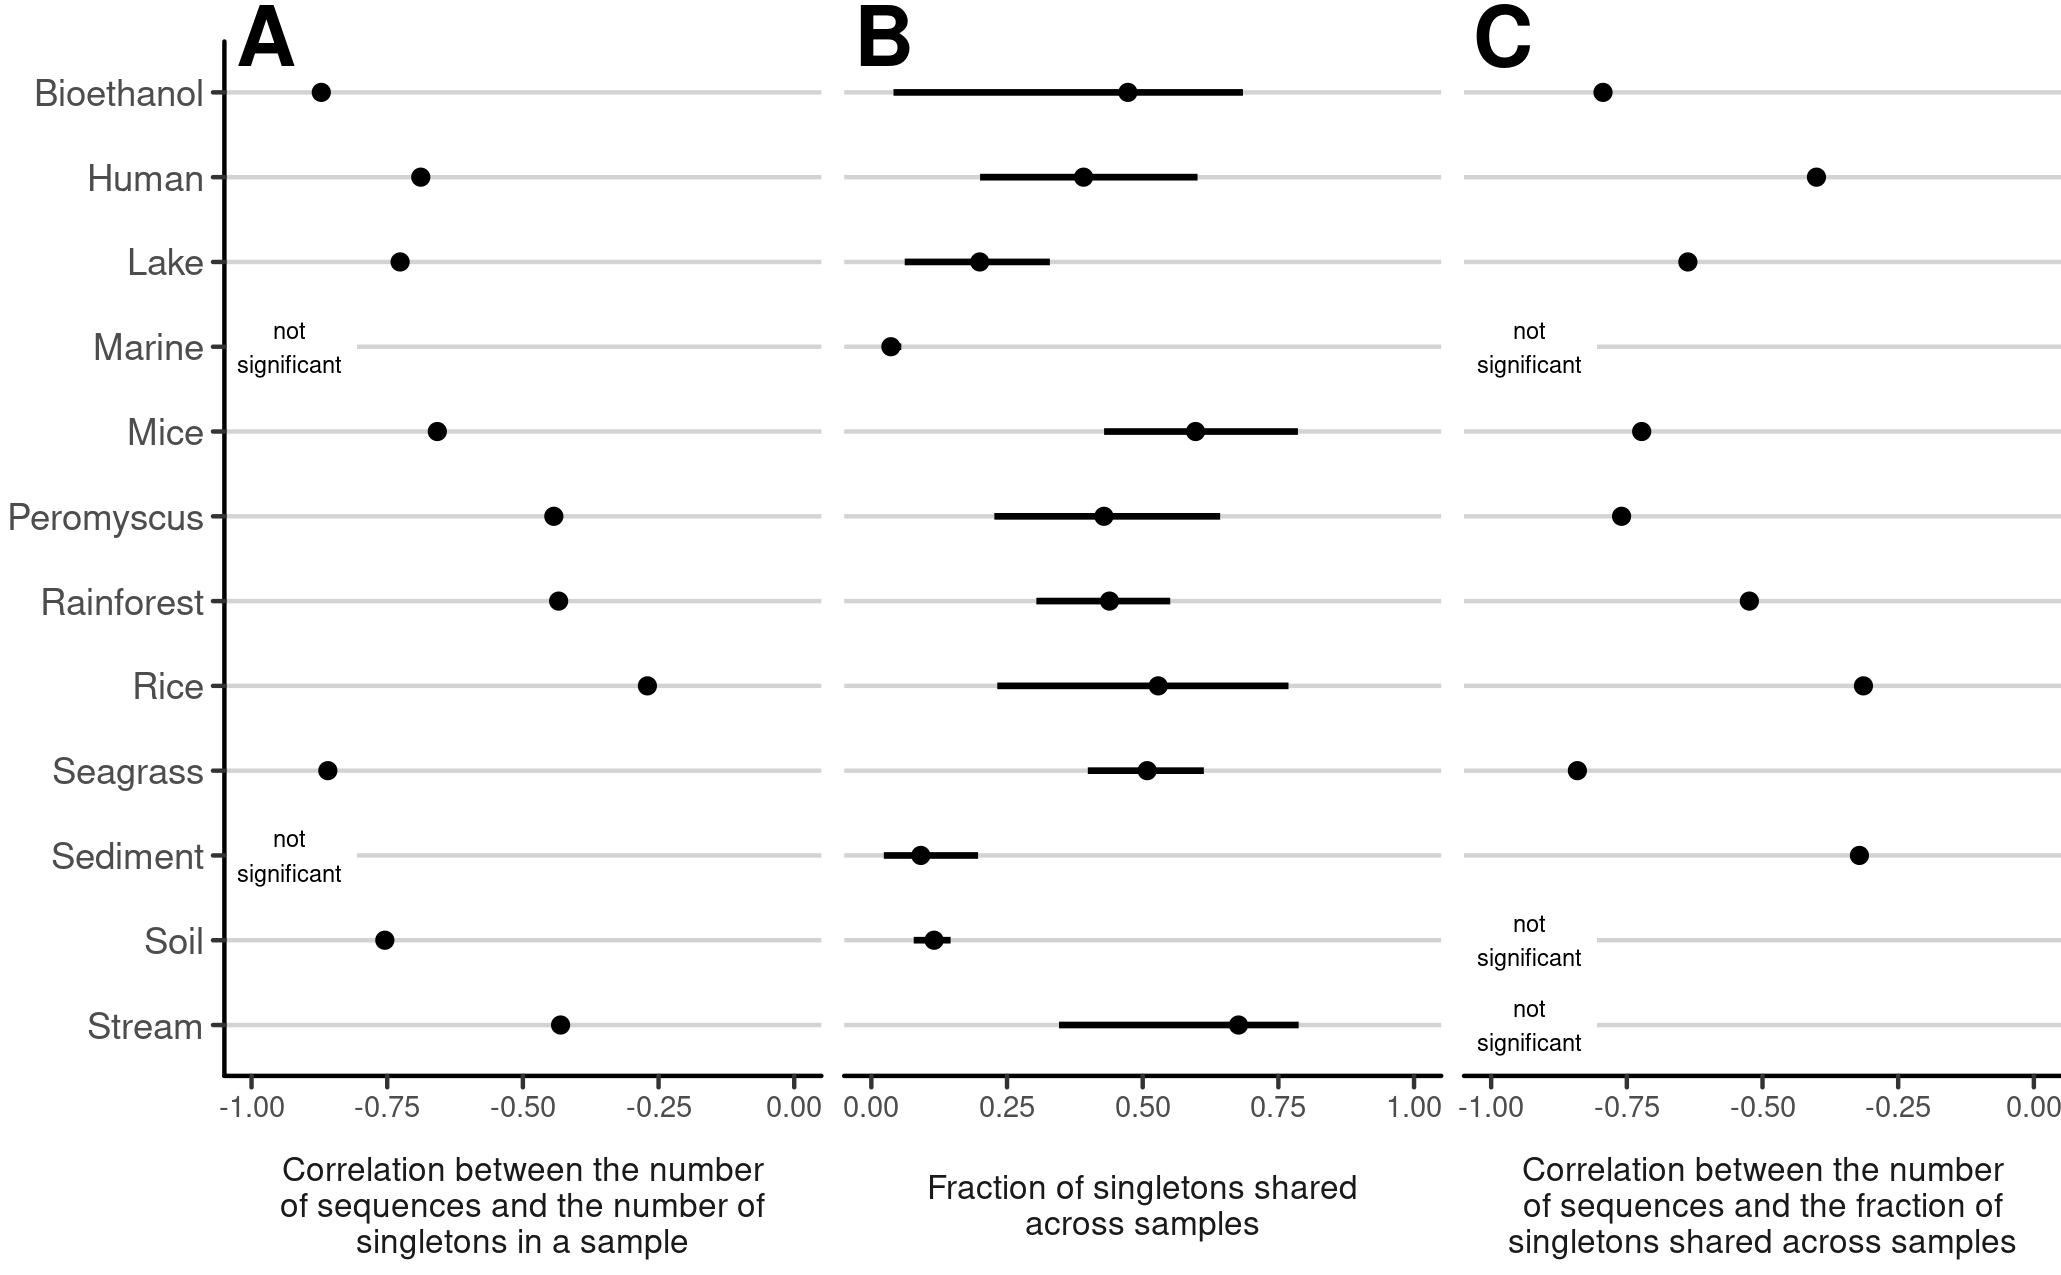
\includegraphics{figure_1.png}

\textbf{Figure 1. Singletons are more common in samples with fewer
seqeunces and tend to be shared with samples having more sequences.} For
each of the 12 datasets, Spearman correlation coefficients were
calcualted between the number of sequences in each sample and the number
of singletons in the sample (A) and the fraction of its singletons that
were shared with another sample (C). Those correlations that were not
statisically significant had a P-value greater than 0.05. The faction of
singletons shared across samples (B) were calculated for each dataset.
The median value is shown with a solid circle and the 95\% confidence
interval is indicated by the solid line.

\newpage

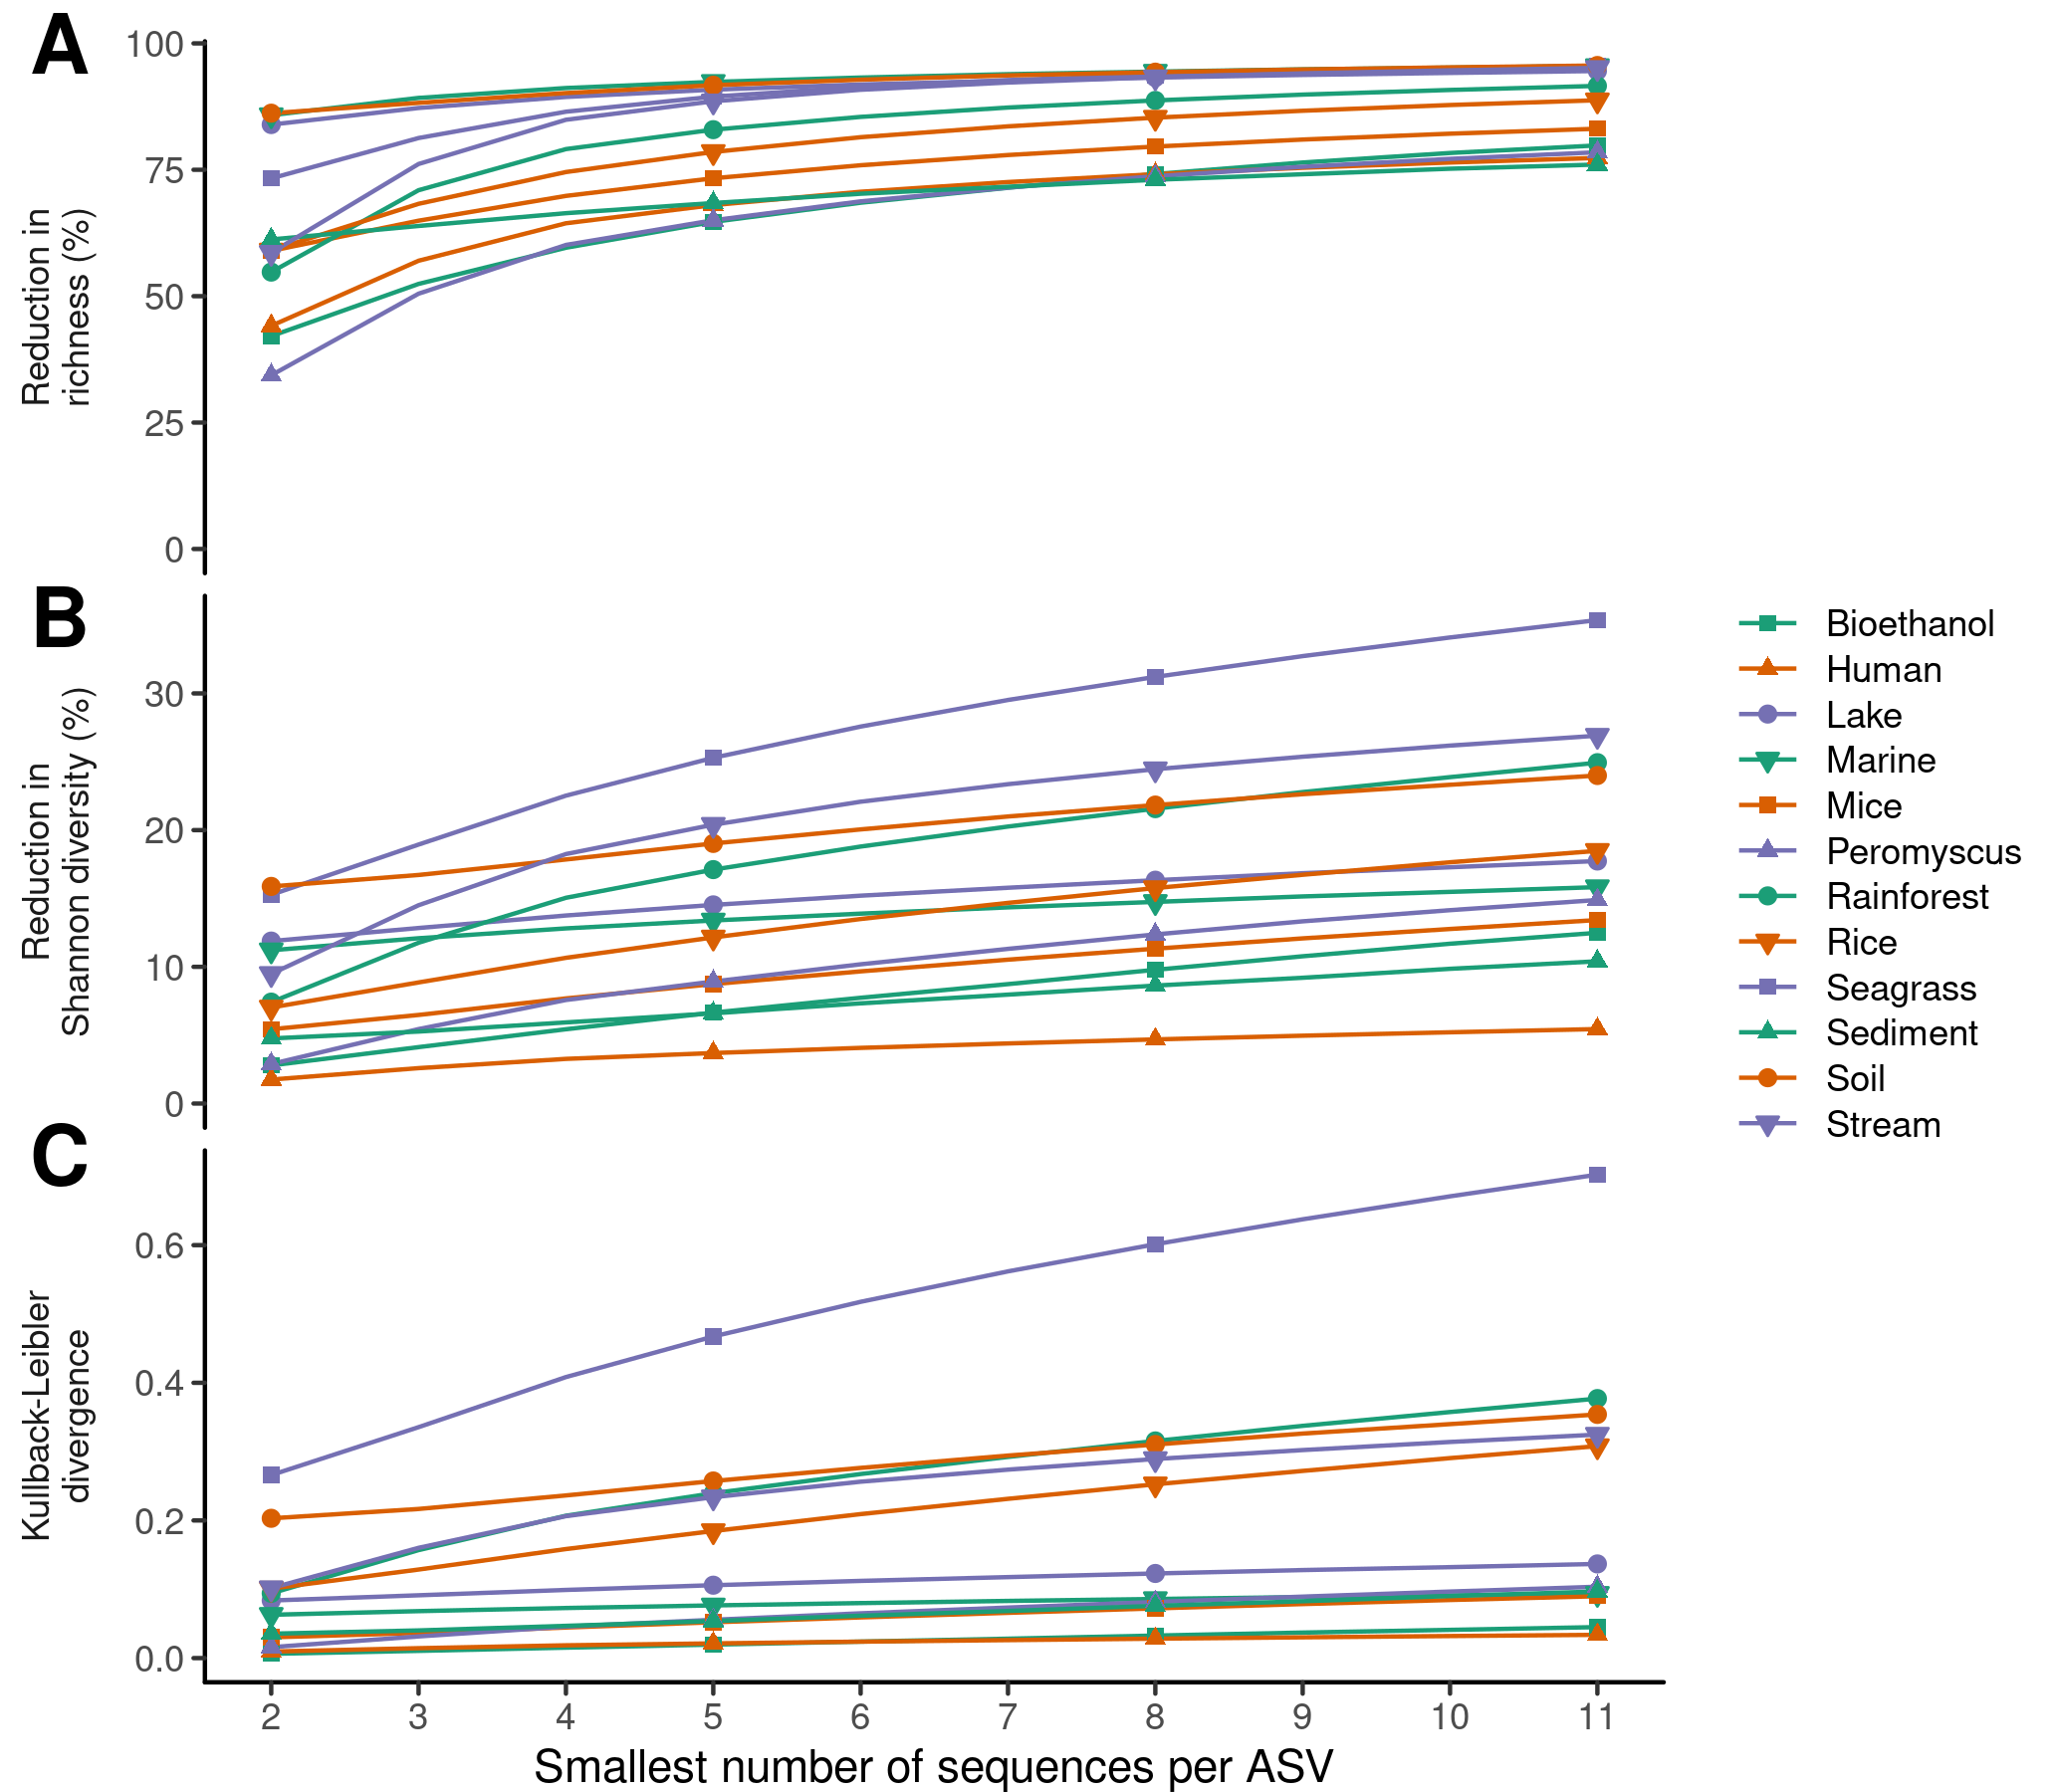
\includegraphics{figure_2.png}

\textbf{Figure 2. Removing rare sequences from samples alters their
representation of alpha-diversity using amplicon sequence variants
(ASVs).} The average difference in the richness (A), Shannon diversity
(B), and Kullback-Leiber divergence (C) for each sample within a dataset
was calculated between the original community structures relative to
applying different minimum abundance thresholds.

\newpage

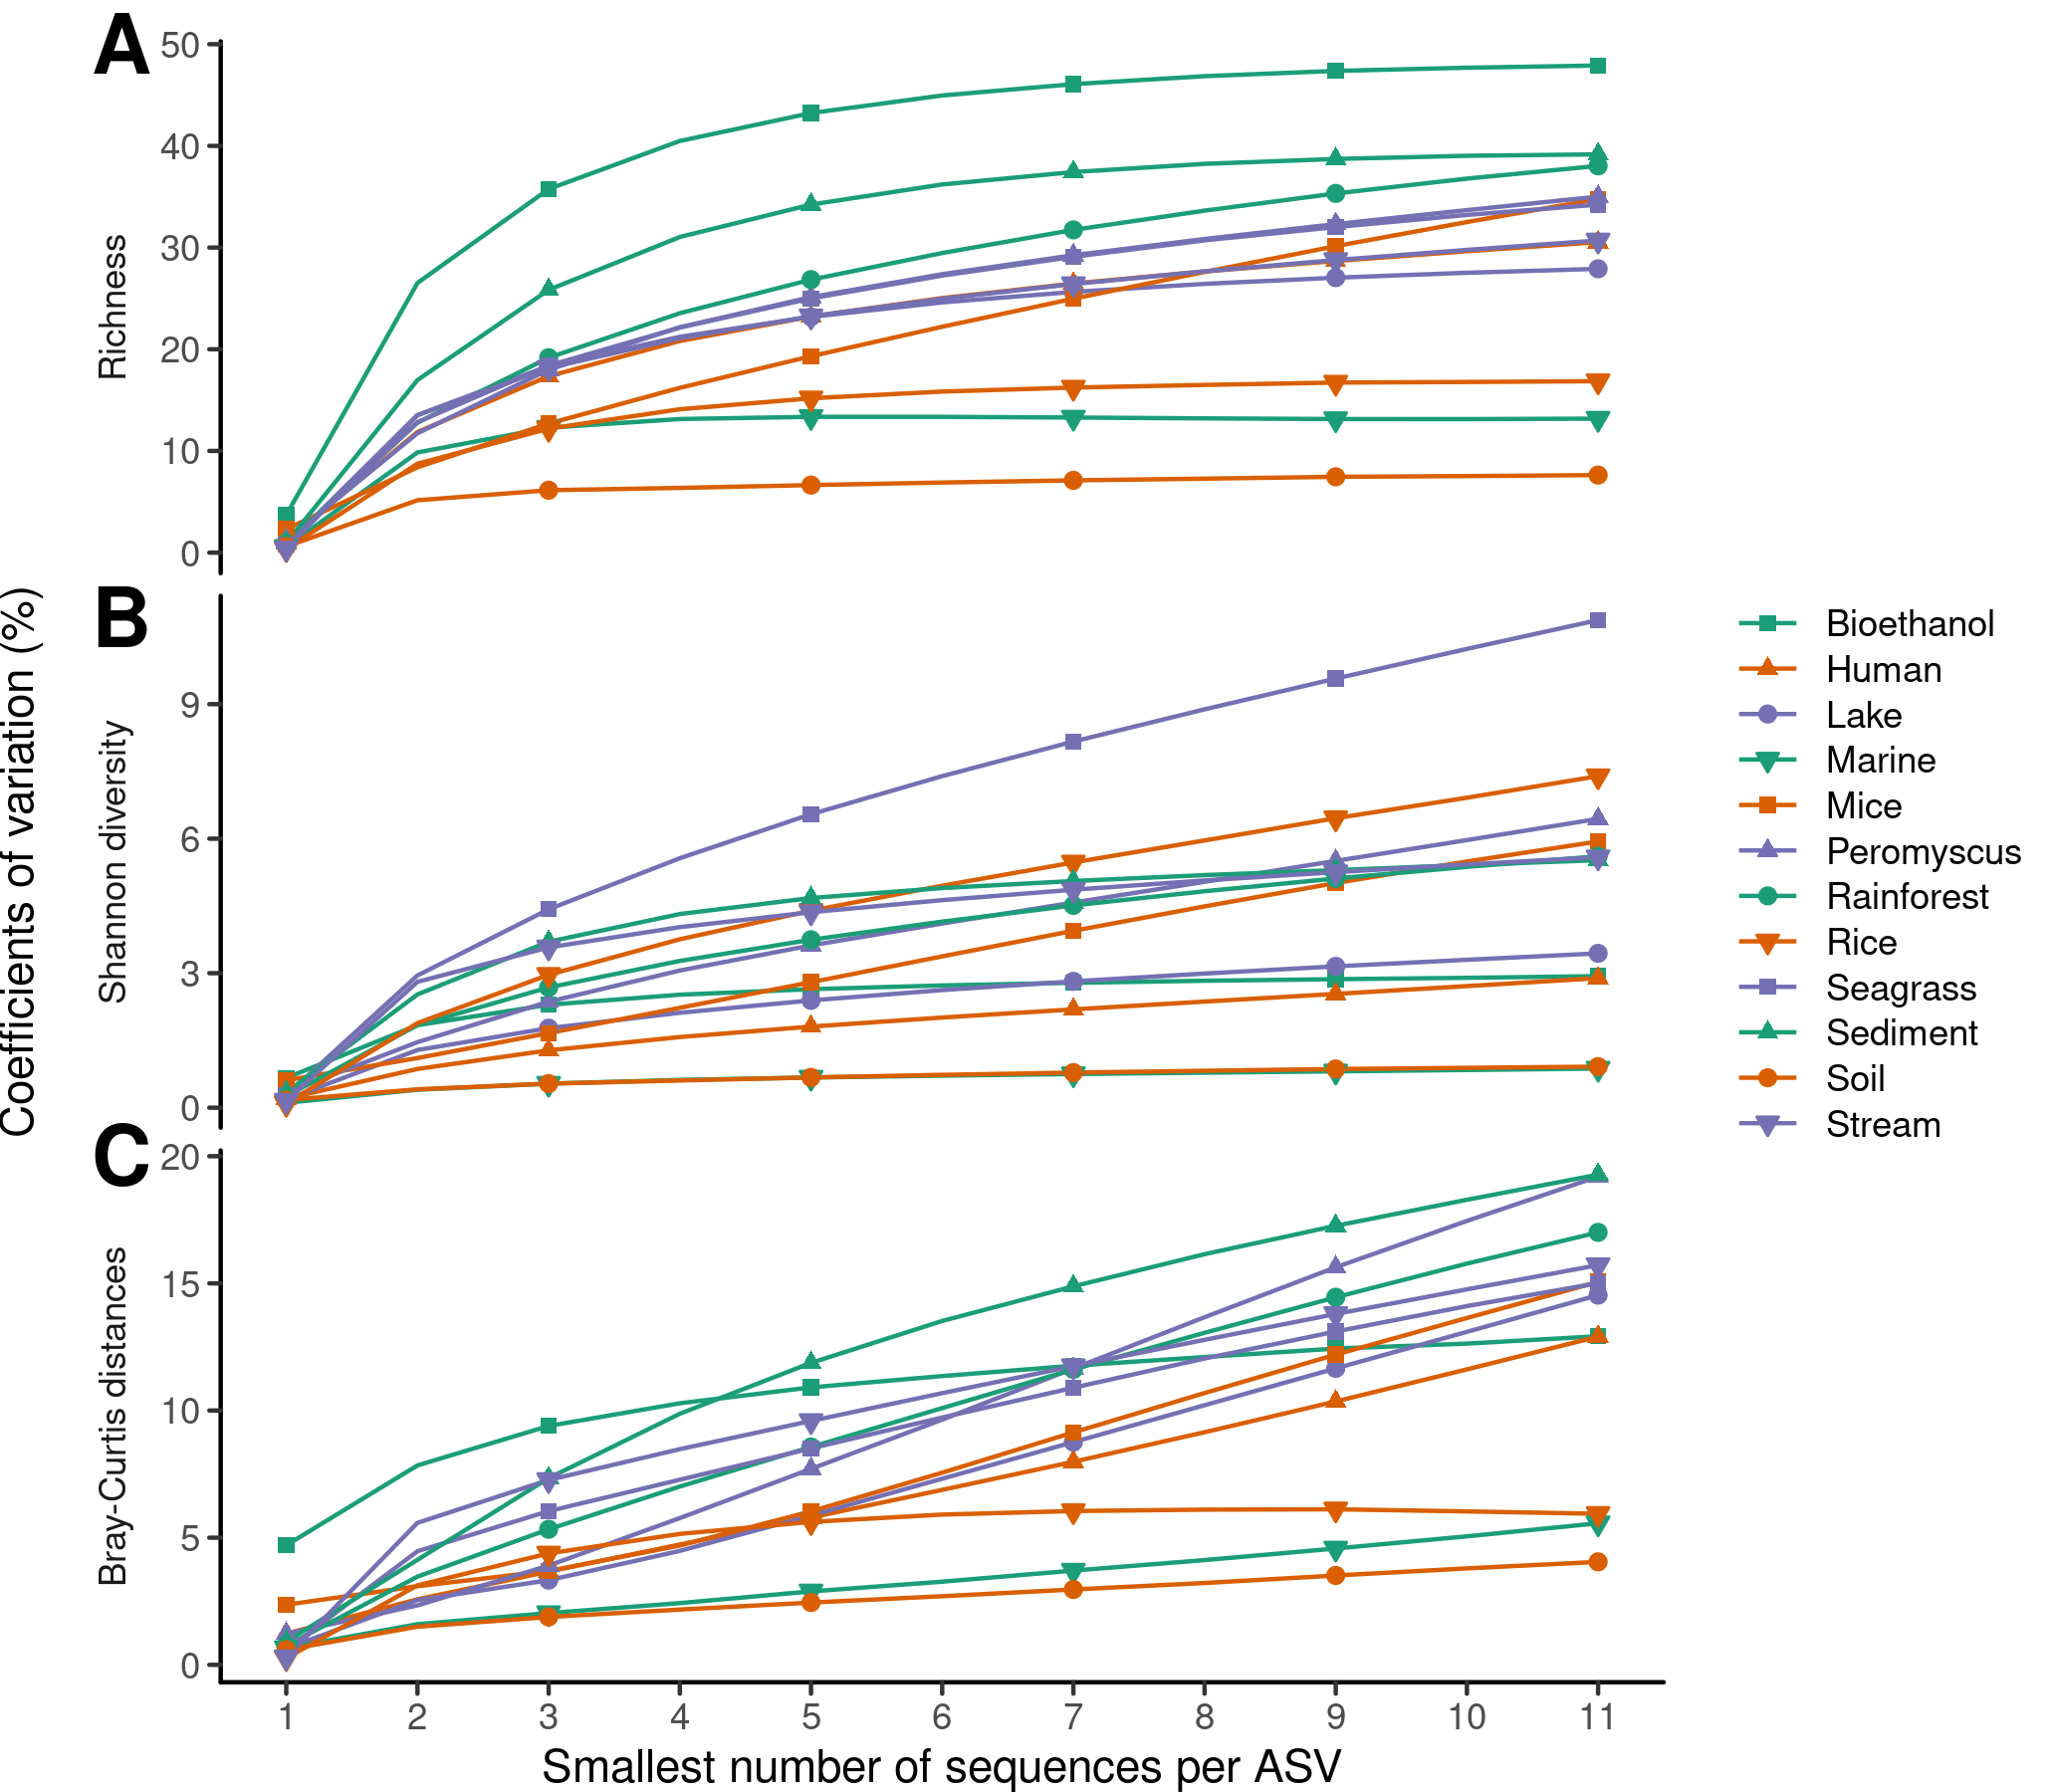
\includegraphics{figure_3.png}

\textbf{Figure 3. Removing rare sequences from samples increases the
inter-sample variation for amplicon sequence variants (ASVs).} The
coefficient of variation in richness (A), Shannon diversity (B), and
Bray-Curtis distances (C) for each dataset was calculated using the null
distributed samples for each dataset with varying minimum abundance
thresholds.

\newpage

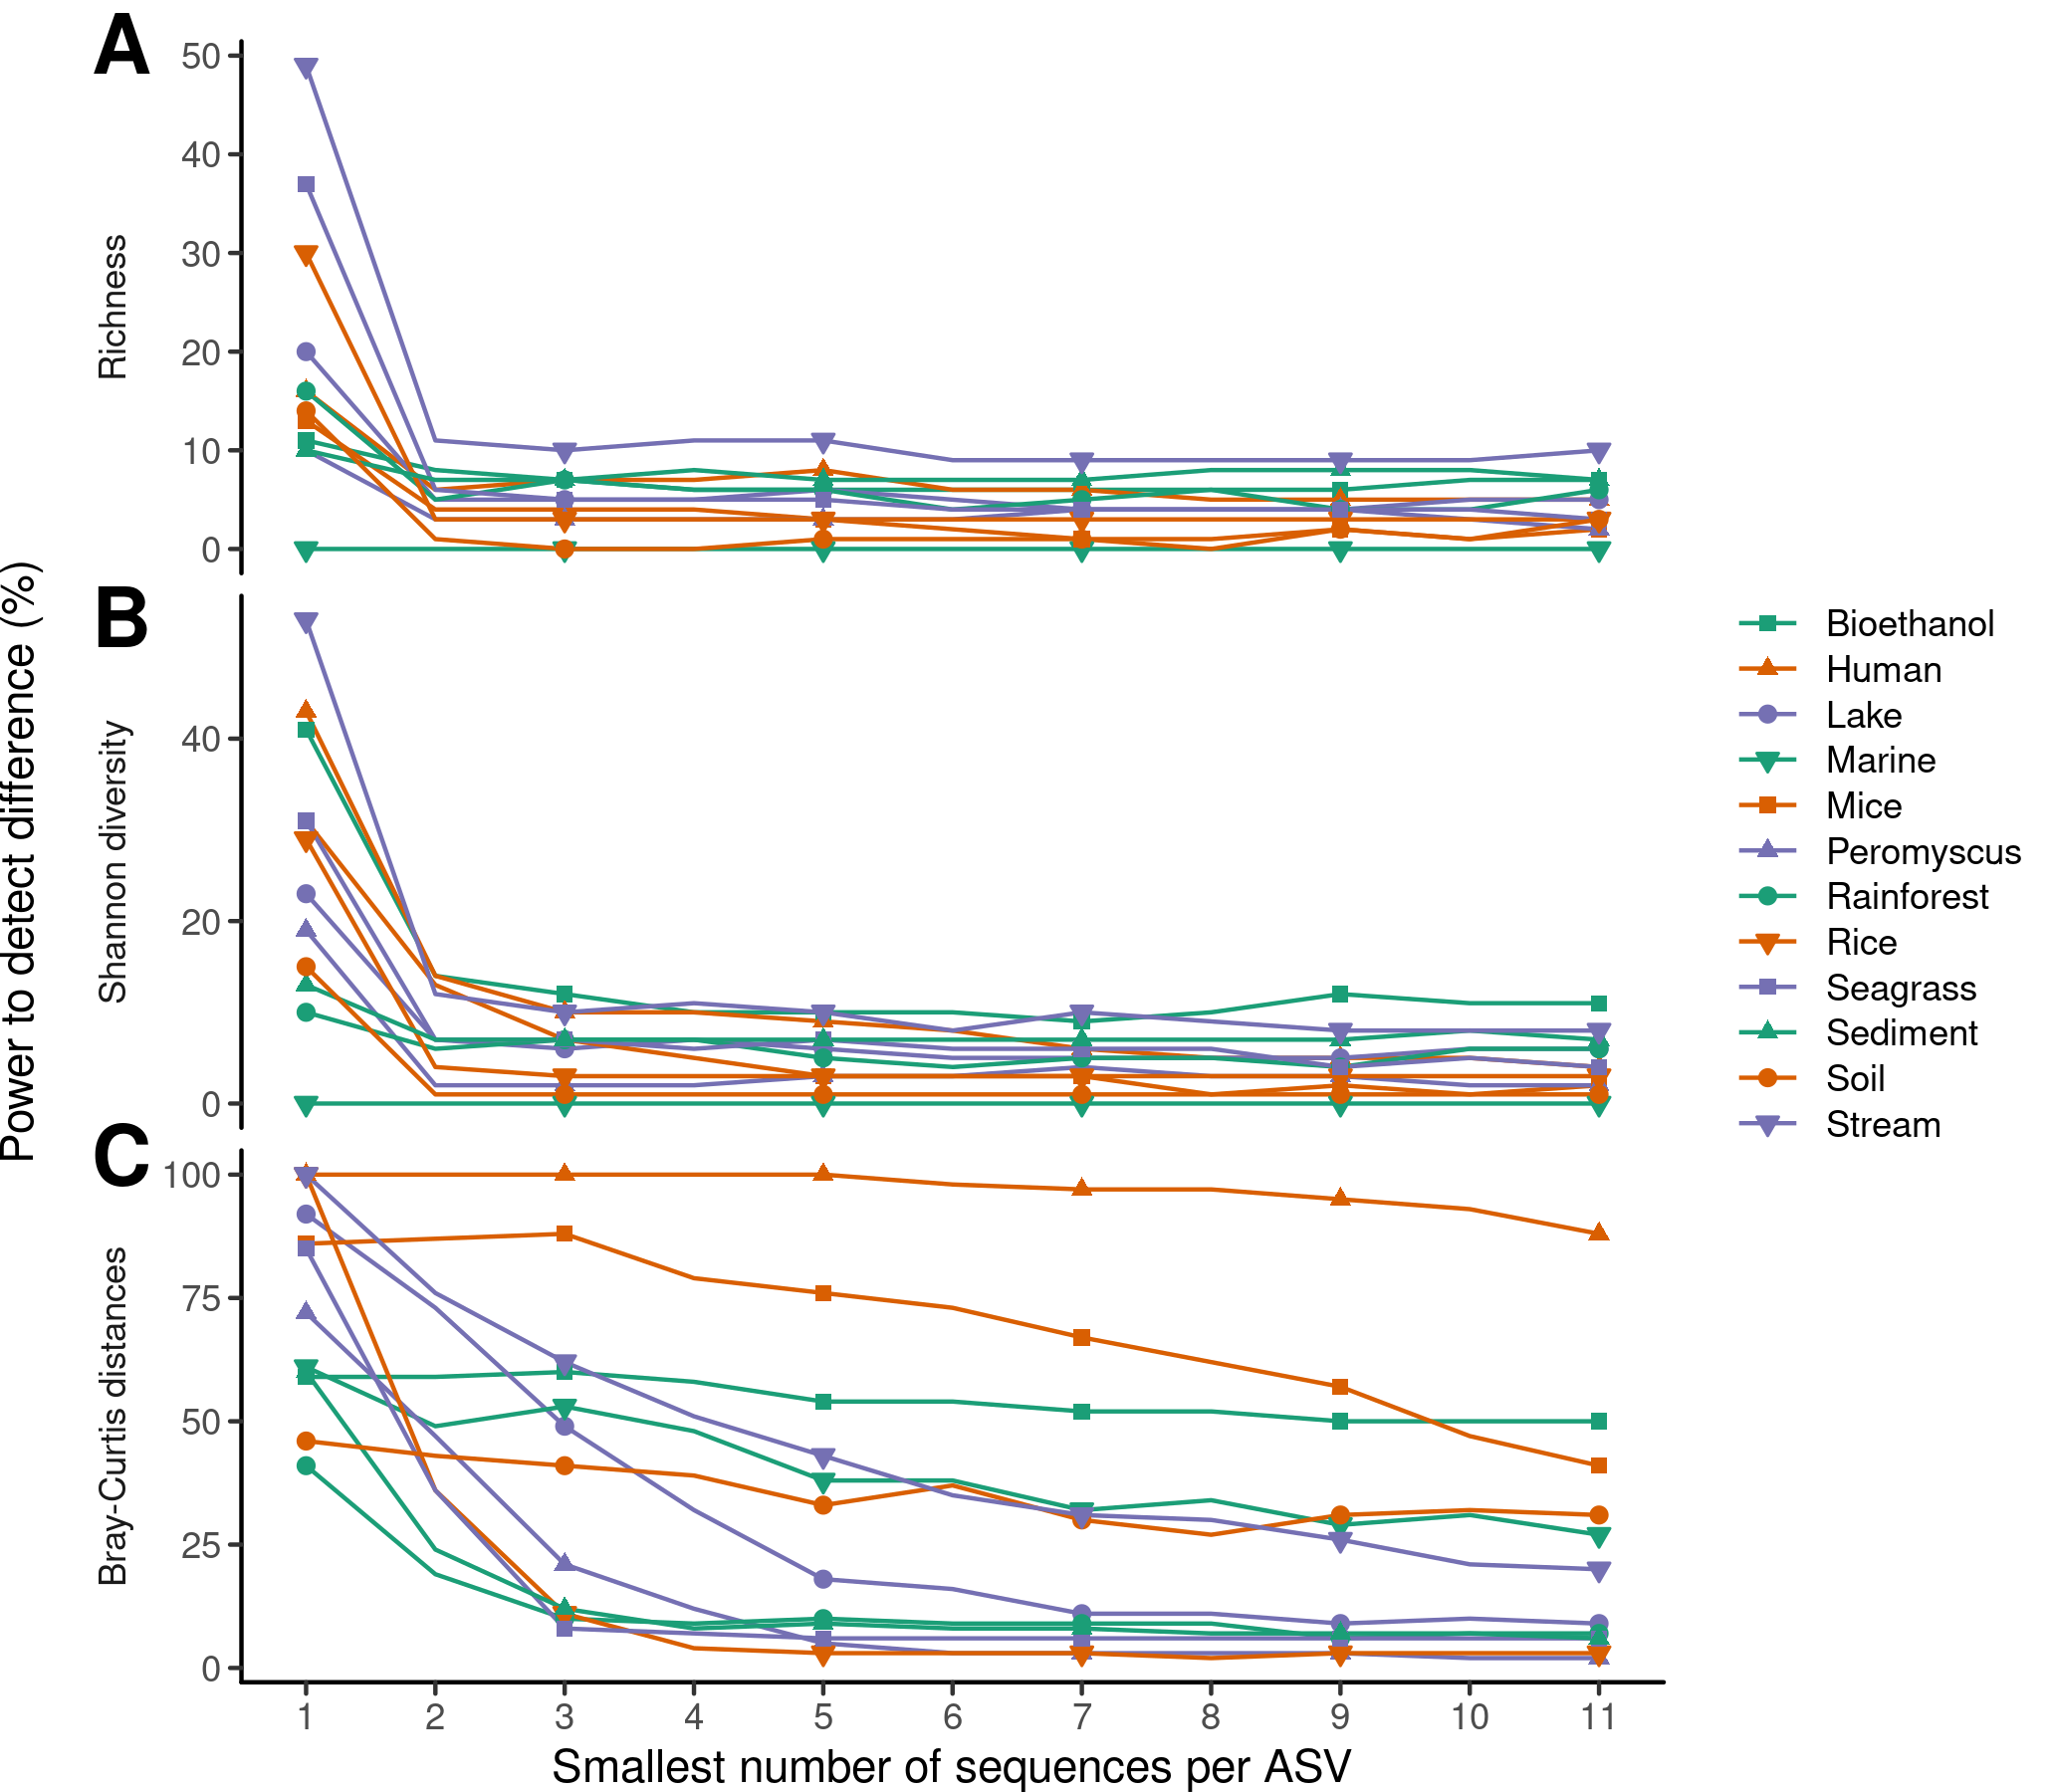
\includegraphics{figure_4.png}

\textbf{Figure 4. Removing rare sequences from samples reduces the
statistical power to detect differences between empirically generated
treatment groups when using amplicon sequence variants (ASVs).} The
fraction of significant tests comparing the richness (A) and Shannon
diversity (B) using a Wilcox test and Bray-Curtis distances (C) using
analysis of molecular variance for each dataset was calculated using
empirically generated treatment groups containing equal numbers of
samples for each dataset with varying minimum abundance thresholds. For
each dataset and minimum abundance threshold, 100 randomizations were
peformed.

\newpage

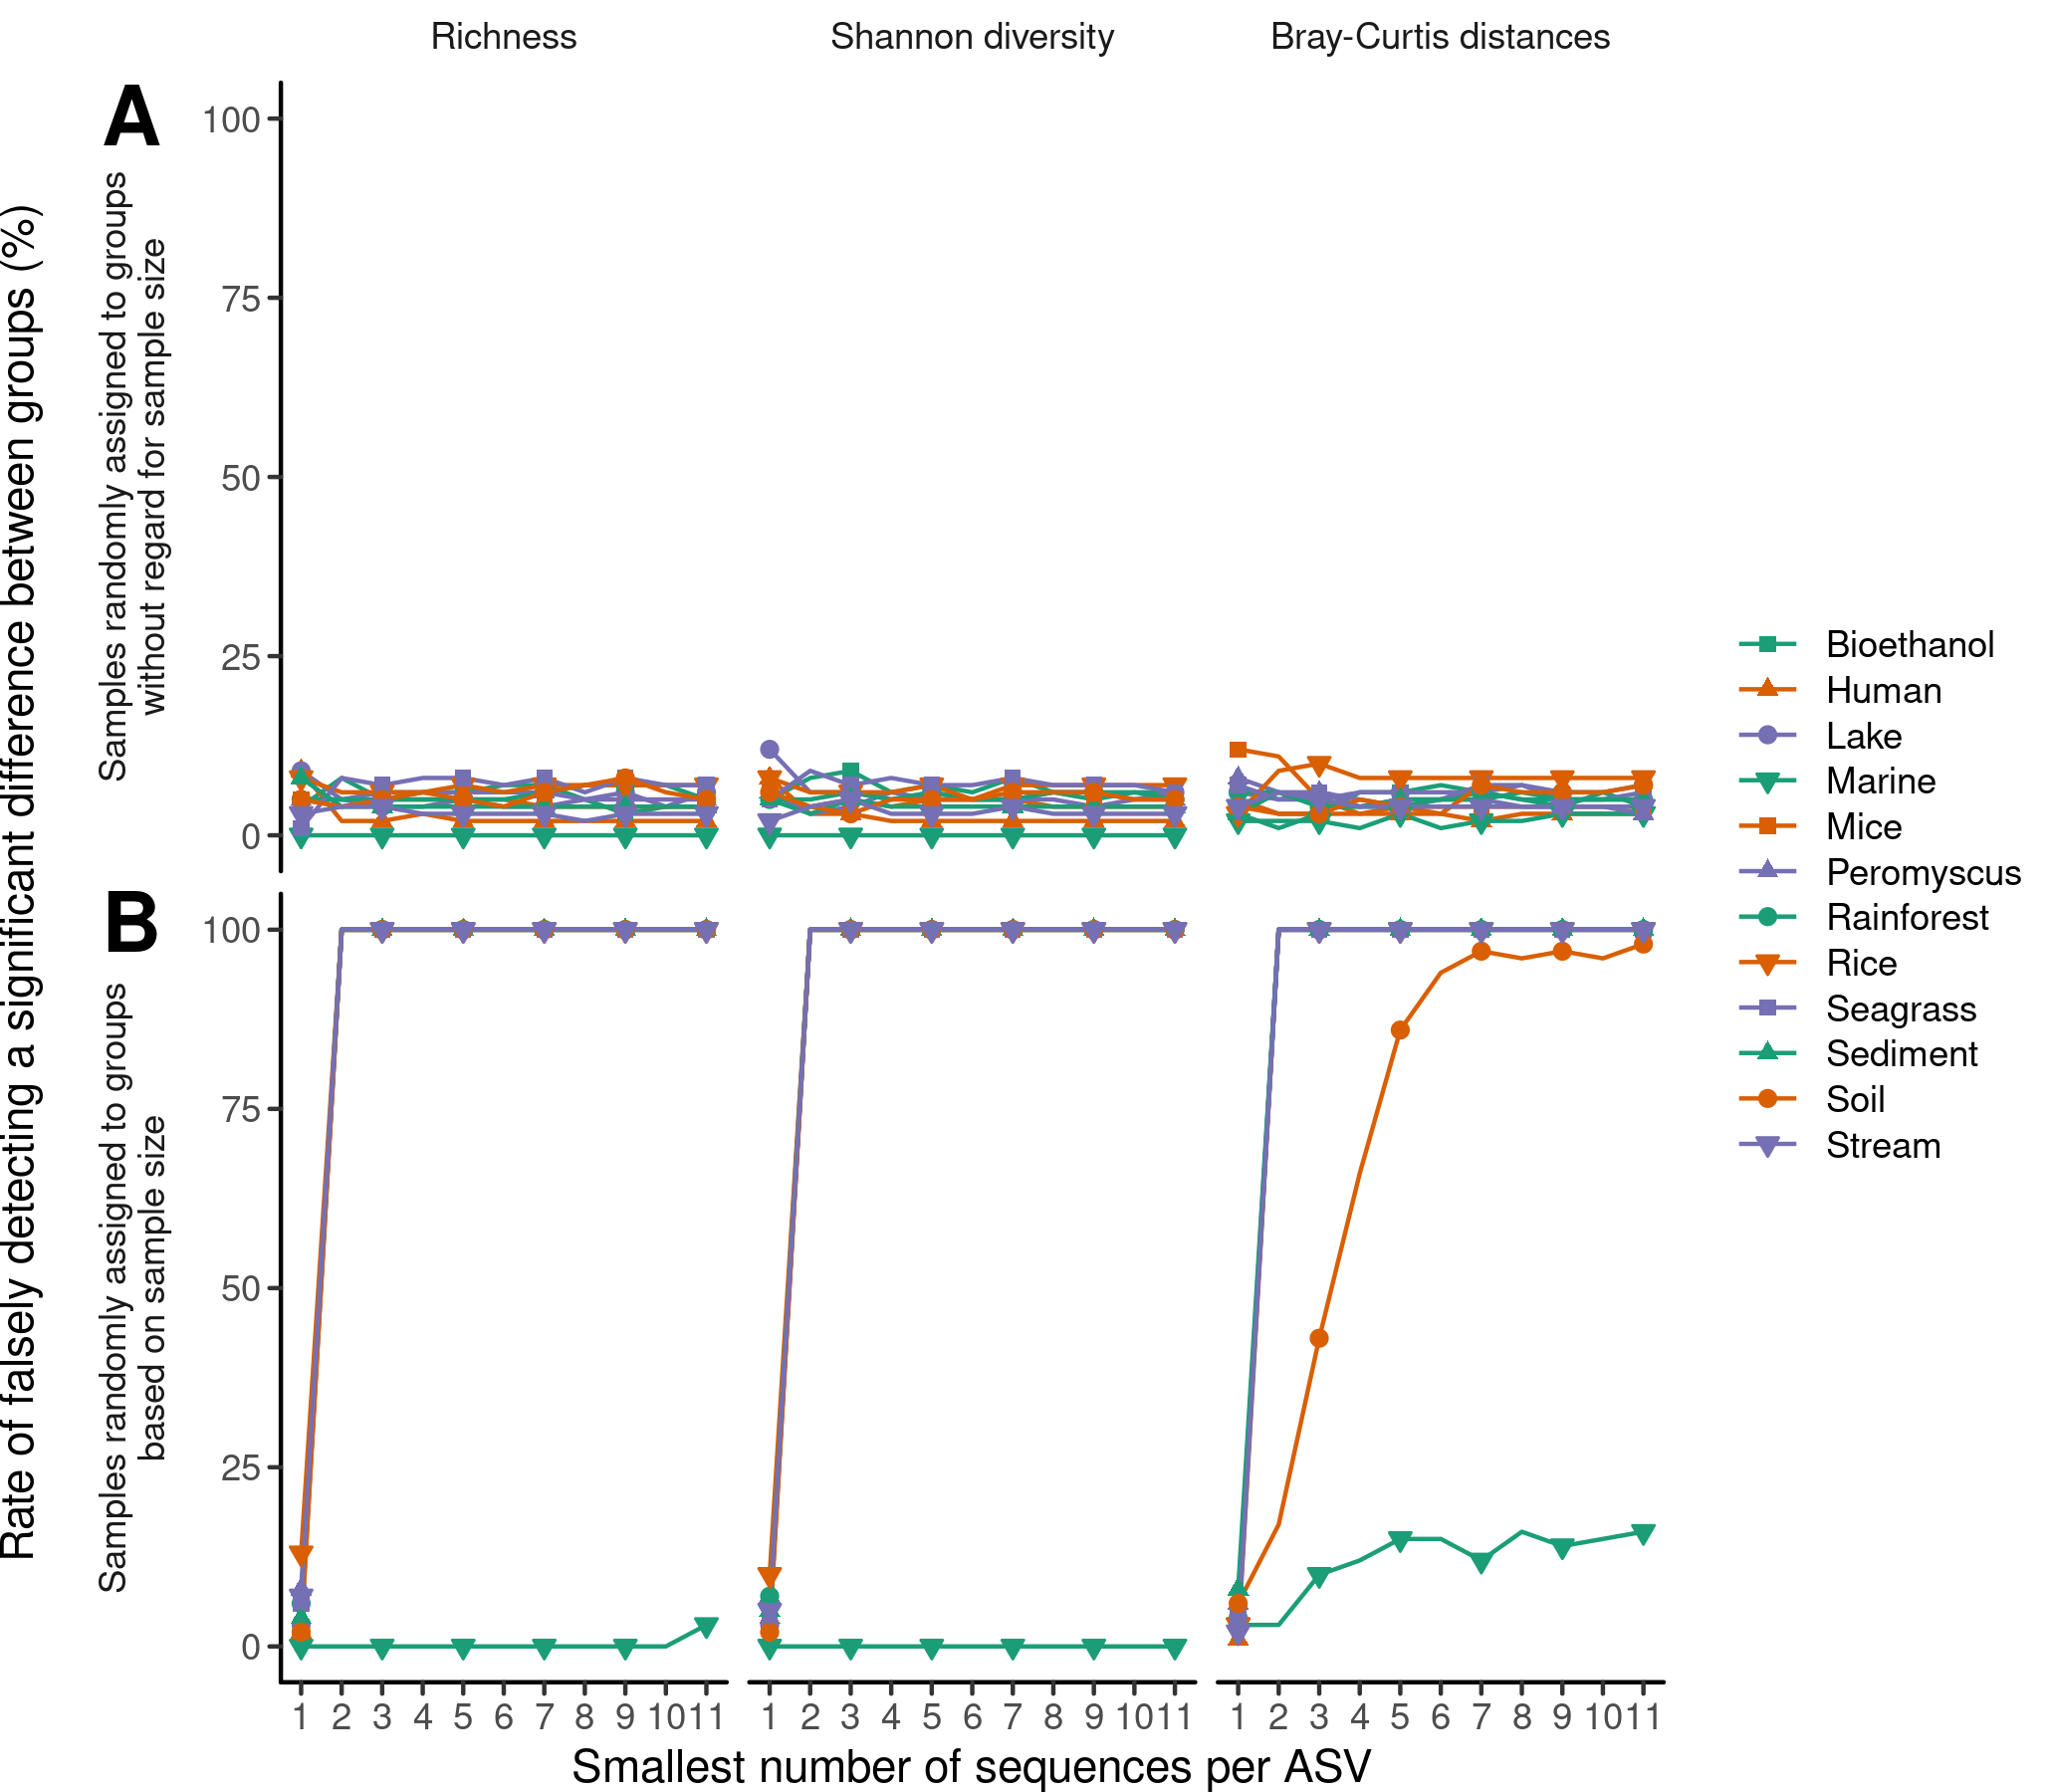
\includegraphics{figure_5.png}

\textbf{Figure 5. Removing rare sequences does not impact the false
detection rate unless the number of sequences per sample is confounded
with the treatment groups when using amplicon sequence variants (ASVs).}
The fraction of significant tests comparing the richness and Shannon
diversity using a Wilcox test and Bray-Curtis distances using analysis
of molecular variance for each dataset was calculated. Empirically
generated treatment groups were generated containing equal numbers of
samples where the samples represented a null distribution. In one
simulation the samples were randomly assigned to a treatment group (A)
and in the other the samples were assigned based on the number of
sequences in each sample (B). For each dataset and minimum abundance
threshold, 100 randomizations were peformed.

\newpage

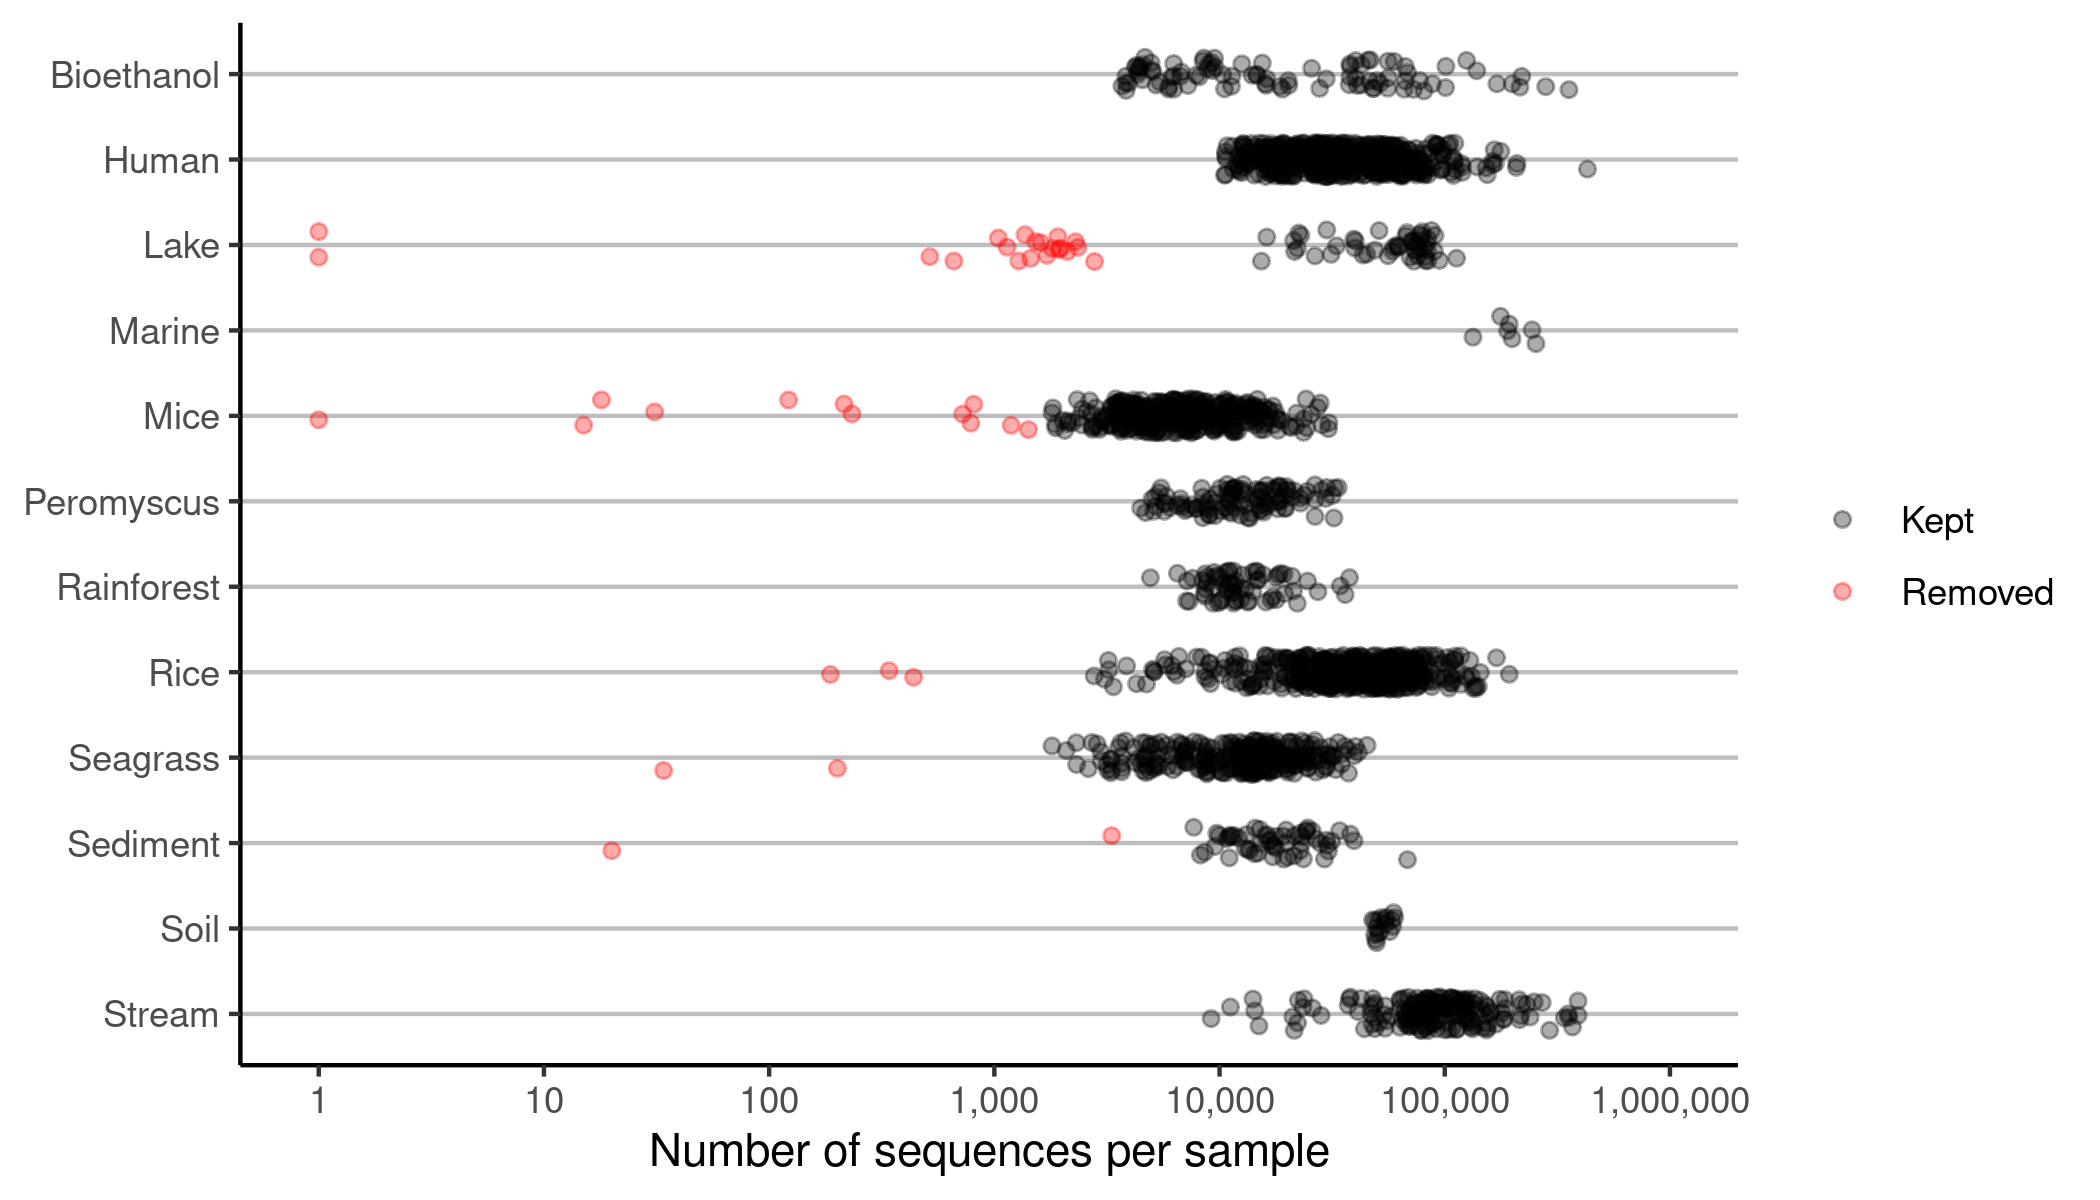
\includegraphics{figure_s1.png}

\textbf{Figure S1. Distribution of the number of sequences per sample in
the 12 datasets included in this study.} A different minimum number of
sequences per sample threshold was applied to each dataset based on
identifying natural breaks in the distribution of the number of
sequences per sample.

\newpage

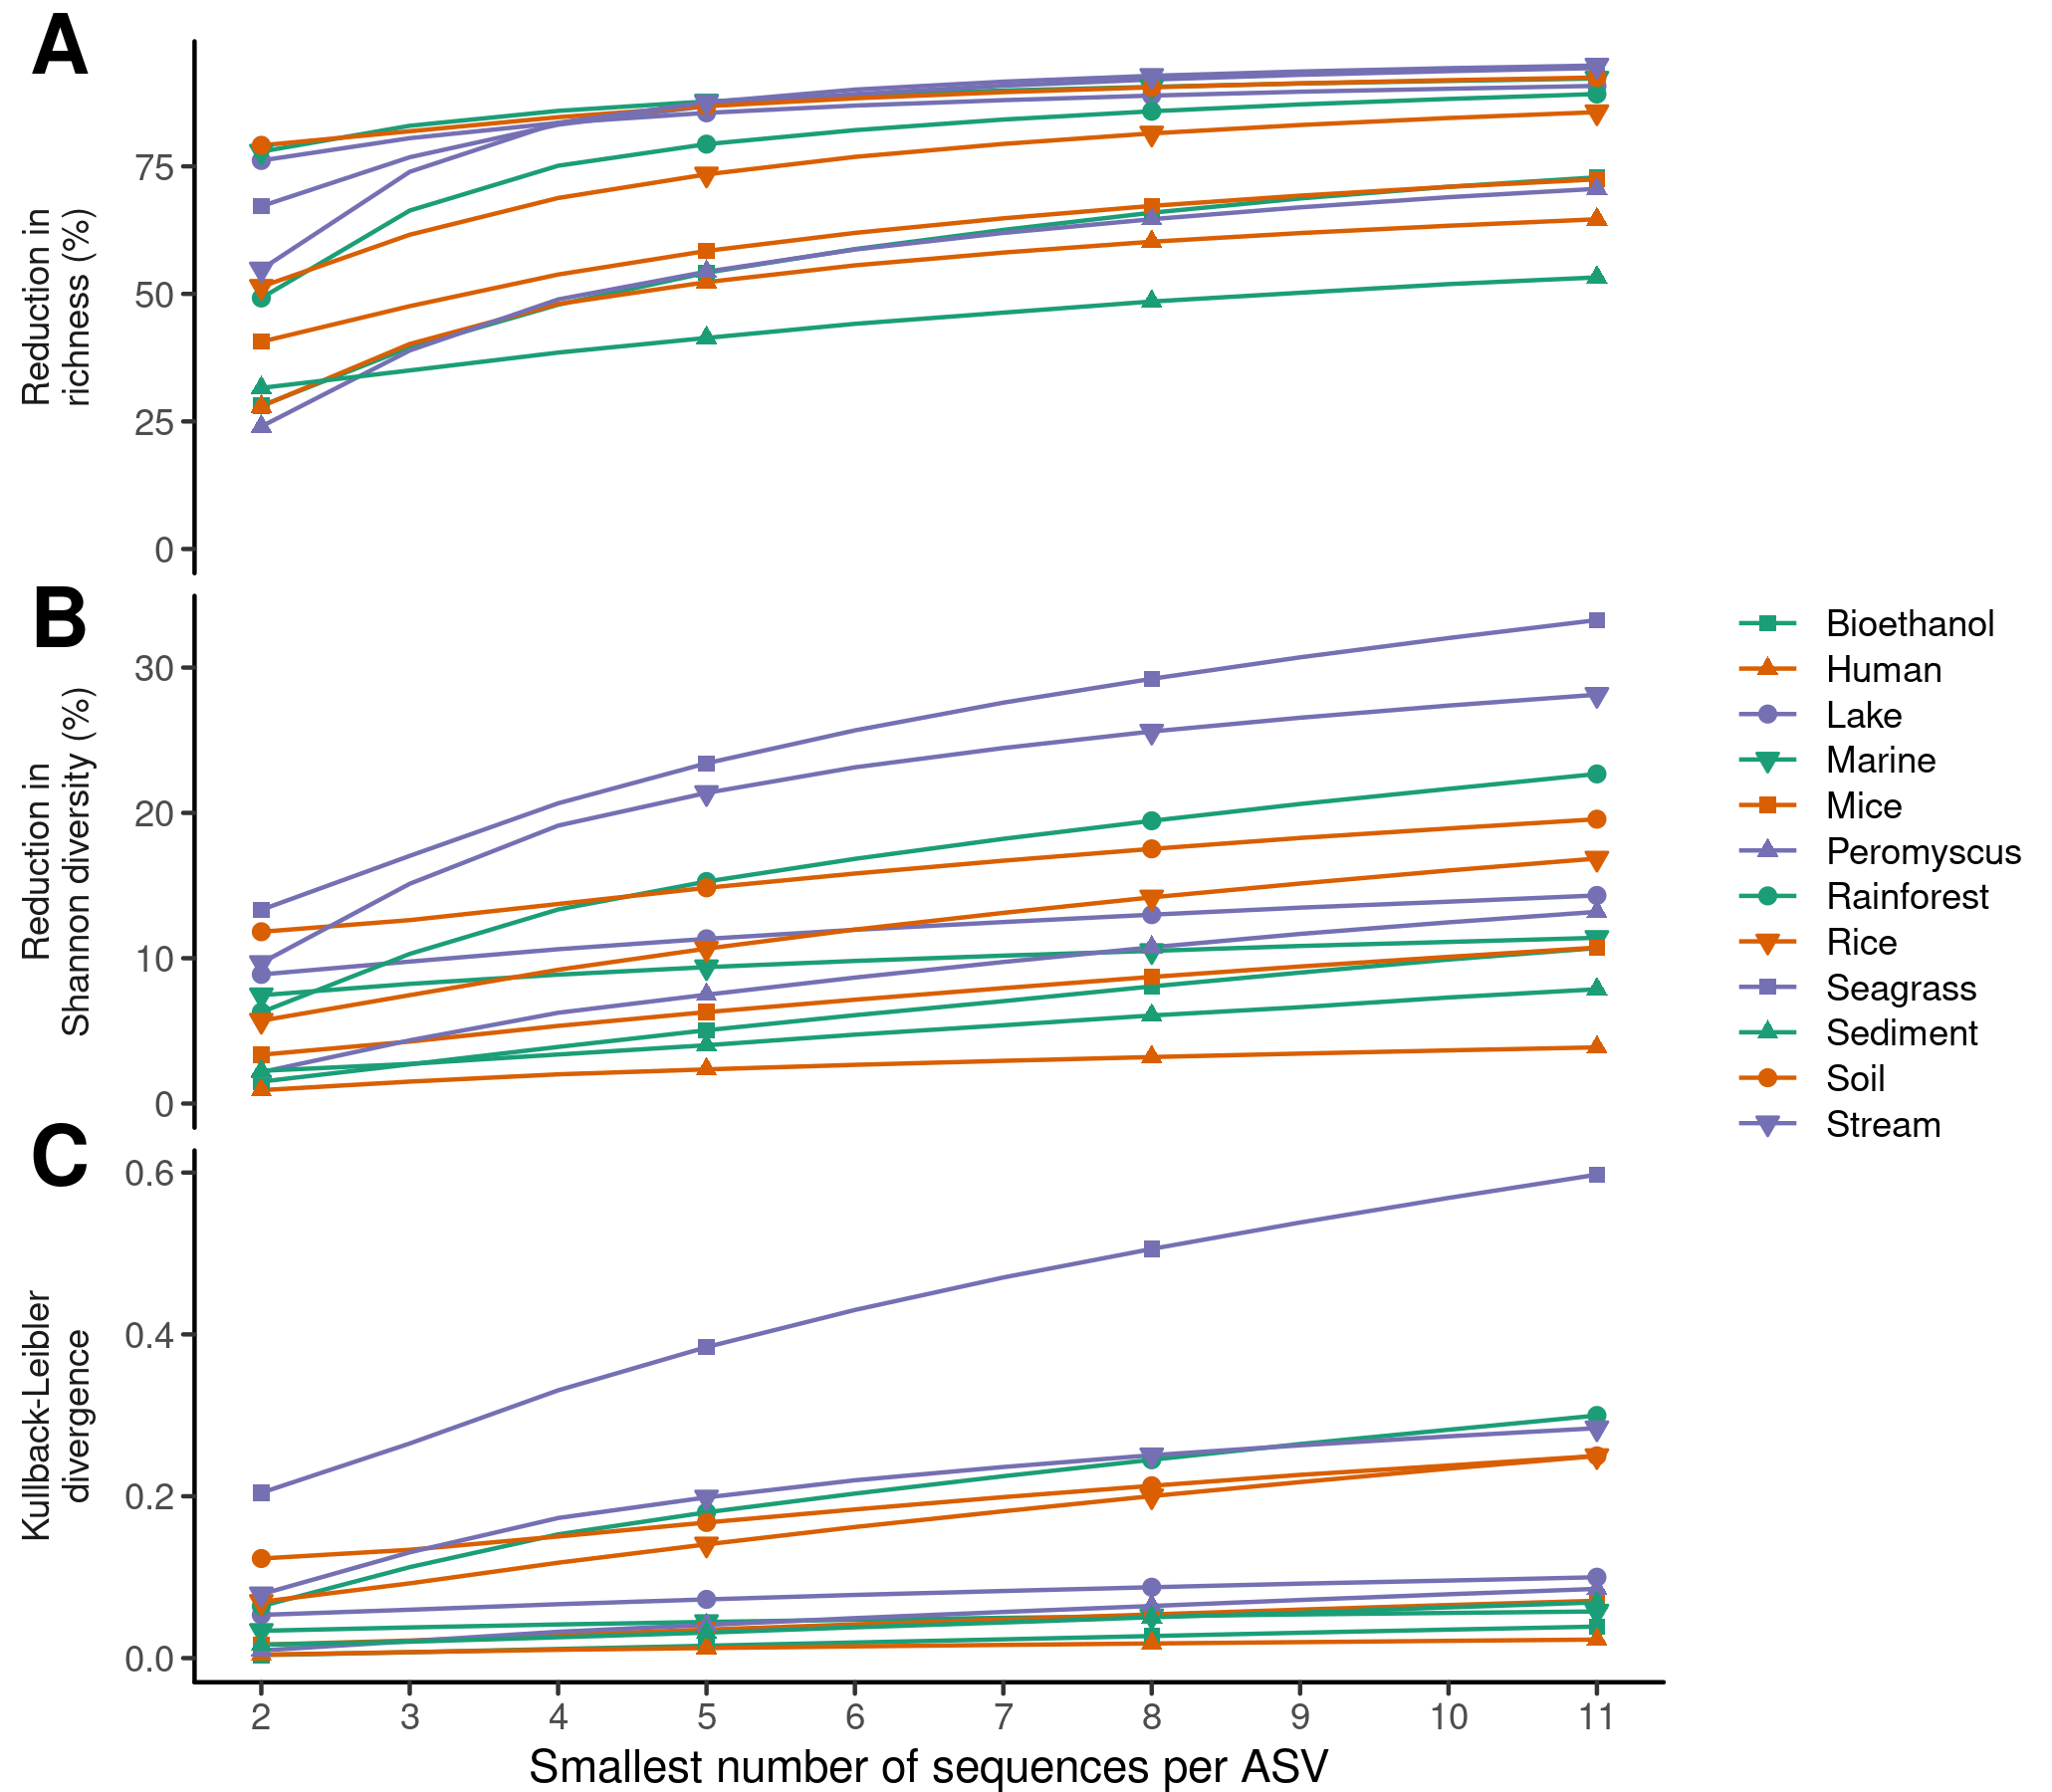
\includegraphics{figure_s2.png}

\textbf{Figure S2. Removing rare sequences from samples alters their
representation of alpha-diversity using operational taxonomic units
(OTUs).} The average difference in the richness (A), Shannon diversity
(B), and Kullback-Leiber divergence (C) for each sample within a dataset
was calculated between the original community structures relative to
applying different minimum abundance thresholds.

\newpage

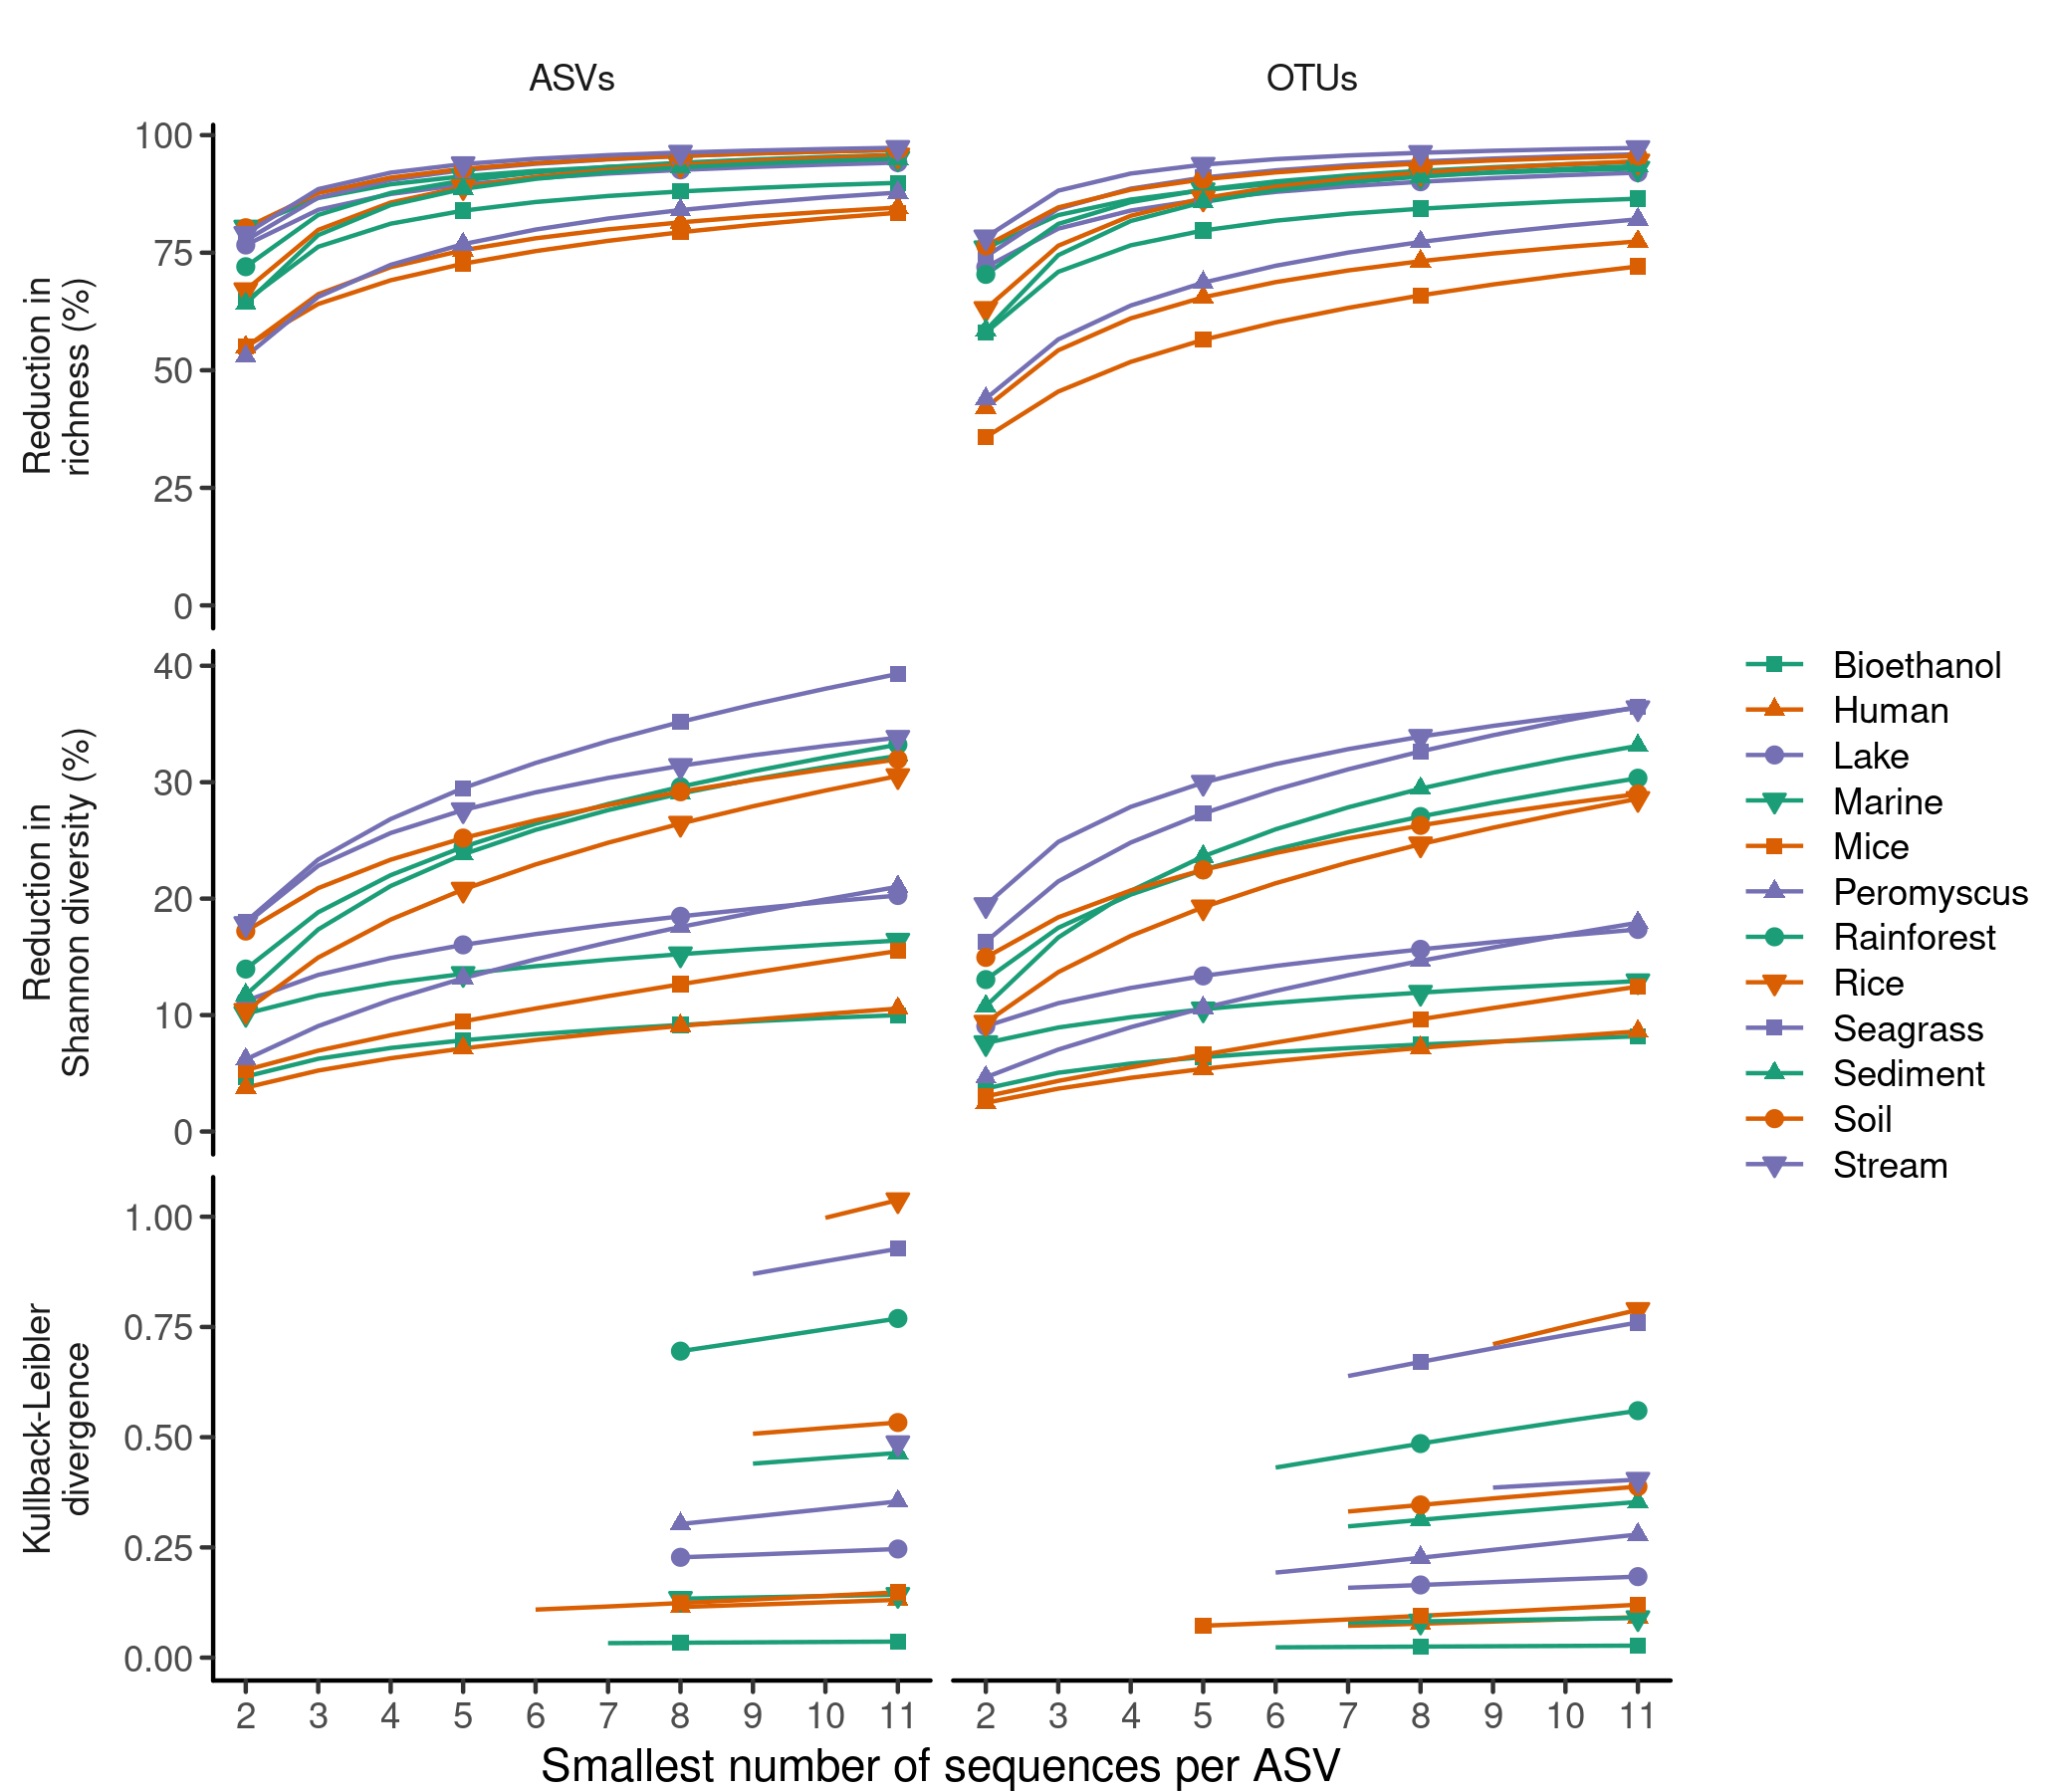
\includegraphics{figure_s3.png}

\textbf{Figure S3. Removing rare sequences from samples alters their
representation of alpha-diversity when regenerating samples using a null
distribution for each dataset.} The average difference in the richness,
Shannon diversity, and Kullback-Leiber divergence for each sample within
a dataset was calculated between the original community structures
relative to applying different minimum abundance thresholds. Some values
of Kullback-Leiber divergence are missing because undefined values were
calculated due to the removal of rare sequences. Data are shown for
amplicon sequence variants (ASVs) and operational taxonomic units (OTUs)

\newpage

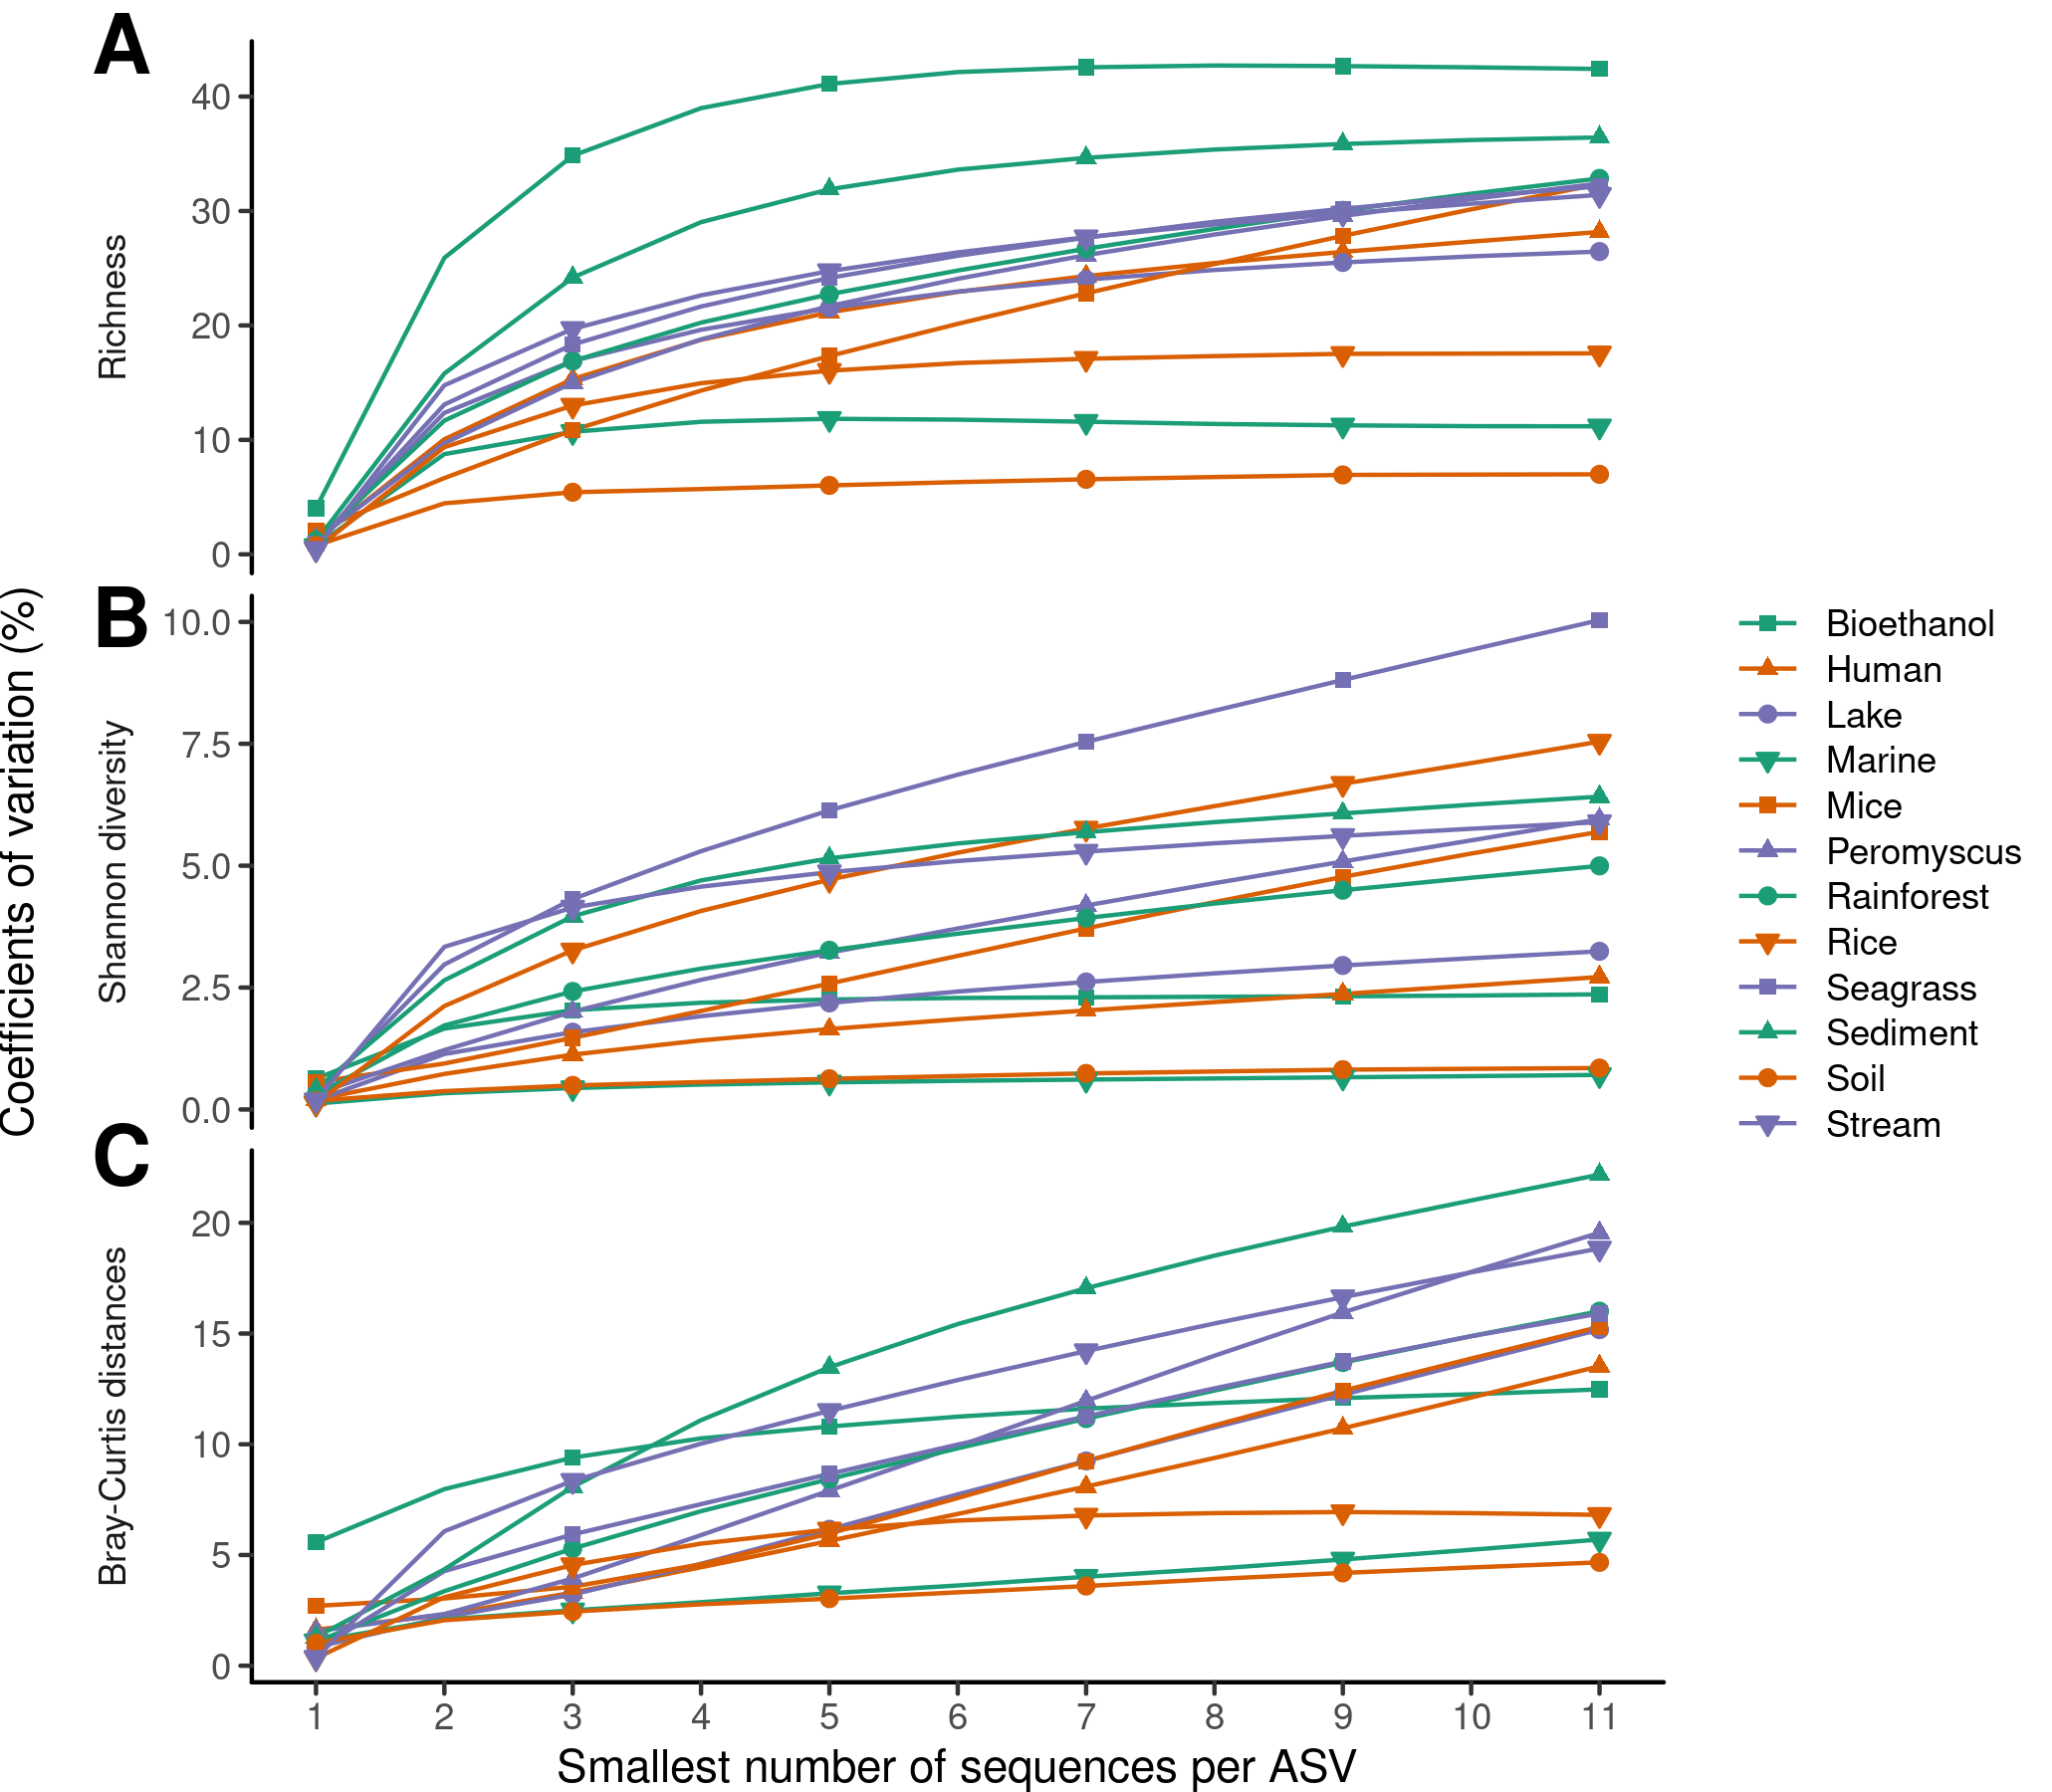
\includegraphics{figure_s4.png}

\textbf{Figure S4. Removing rare sequences from samples increases the
inter-sample variation for operational taxonomic units (OTUs).} The
coefficient of variation in richness (A), Shannon diversity (B), and
Bray-Curtis distances (C) for each dataset was calculated using the null
distributed samples for each dataset with varying minimum abundance
thresholds.

\newpage

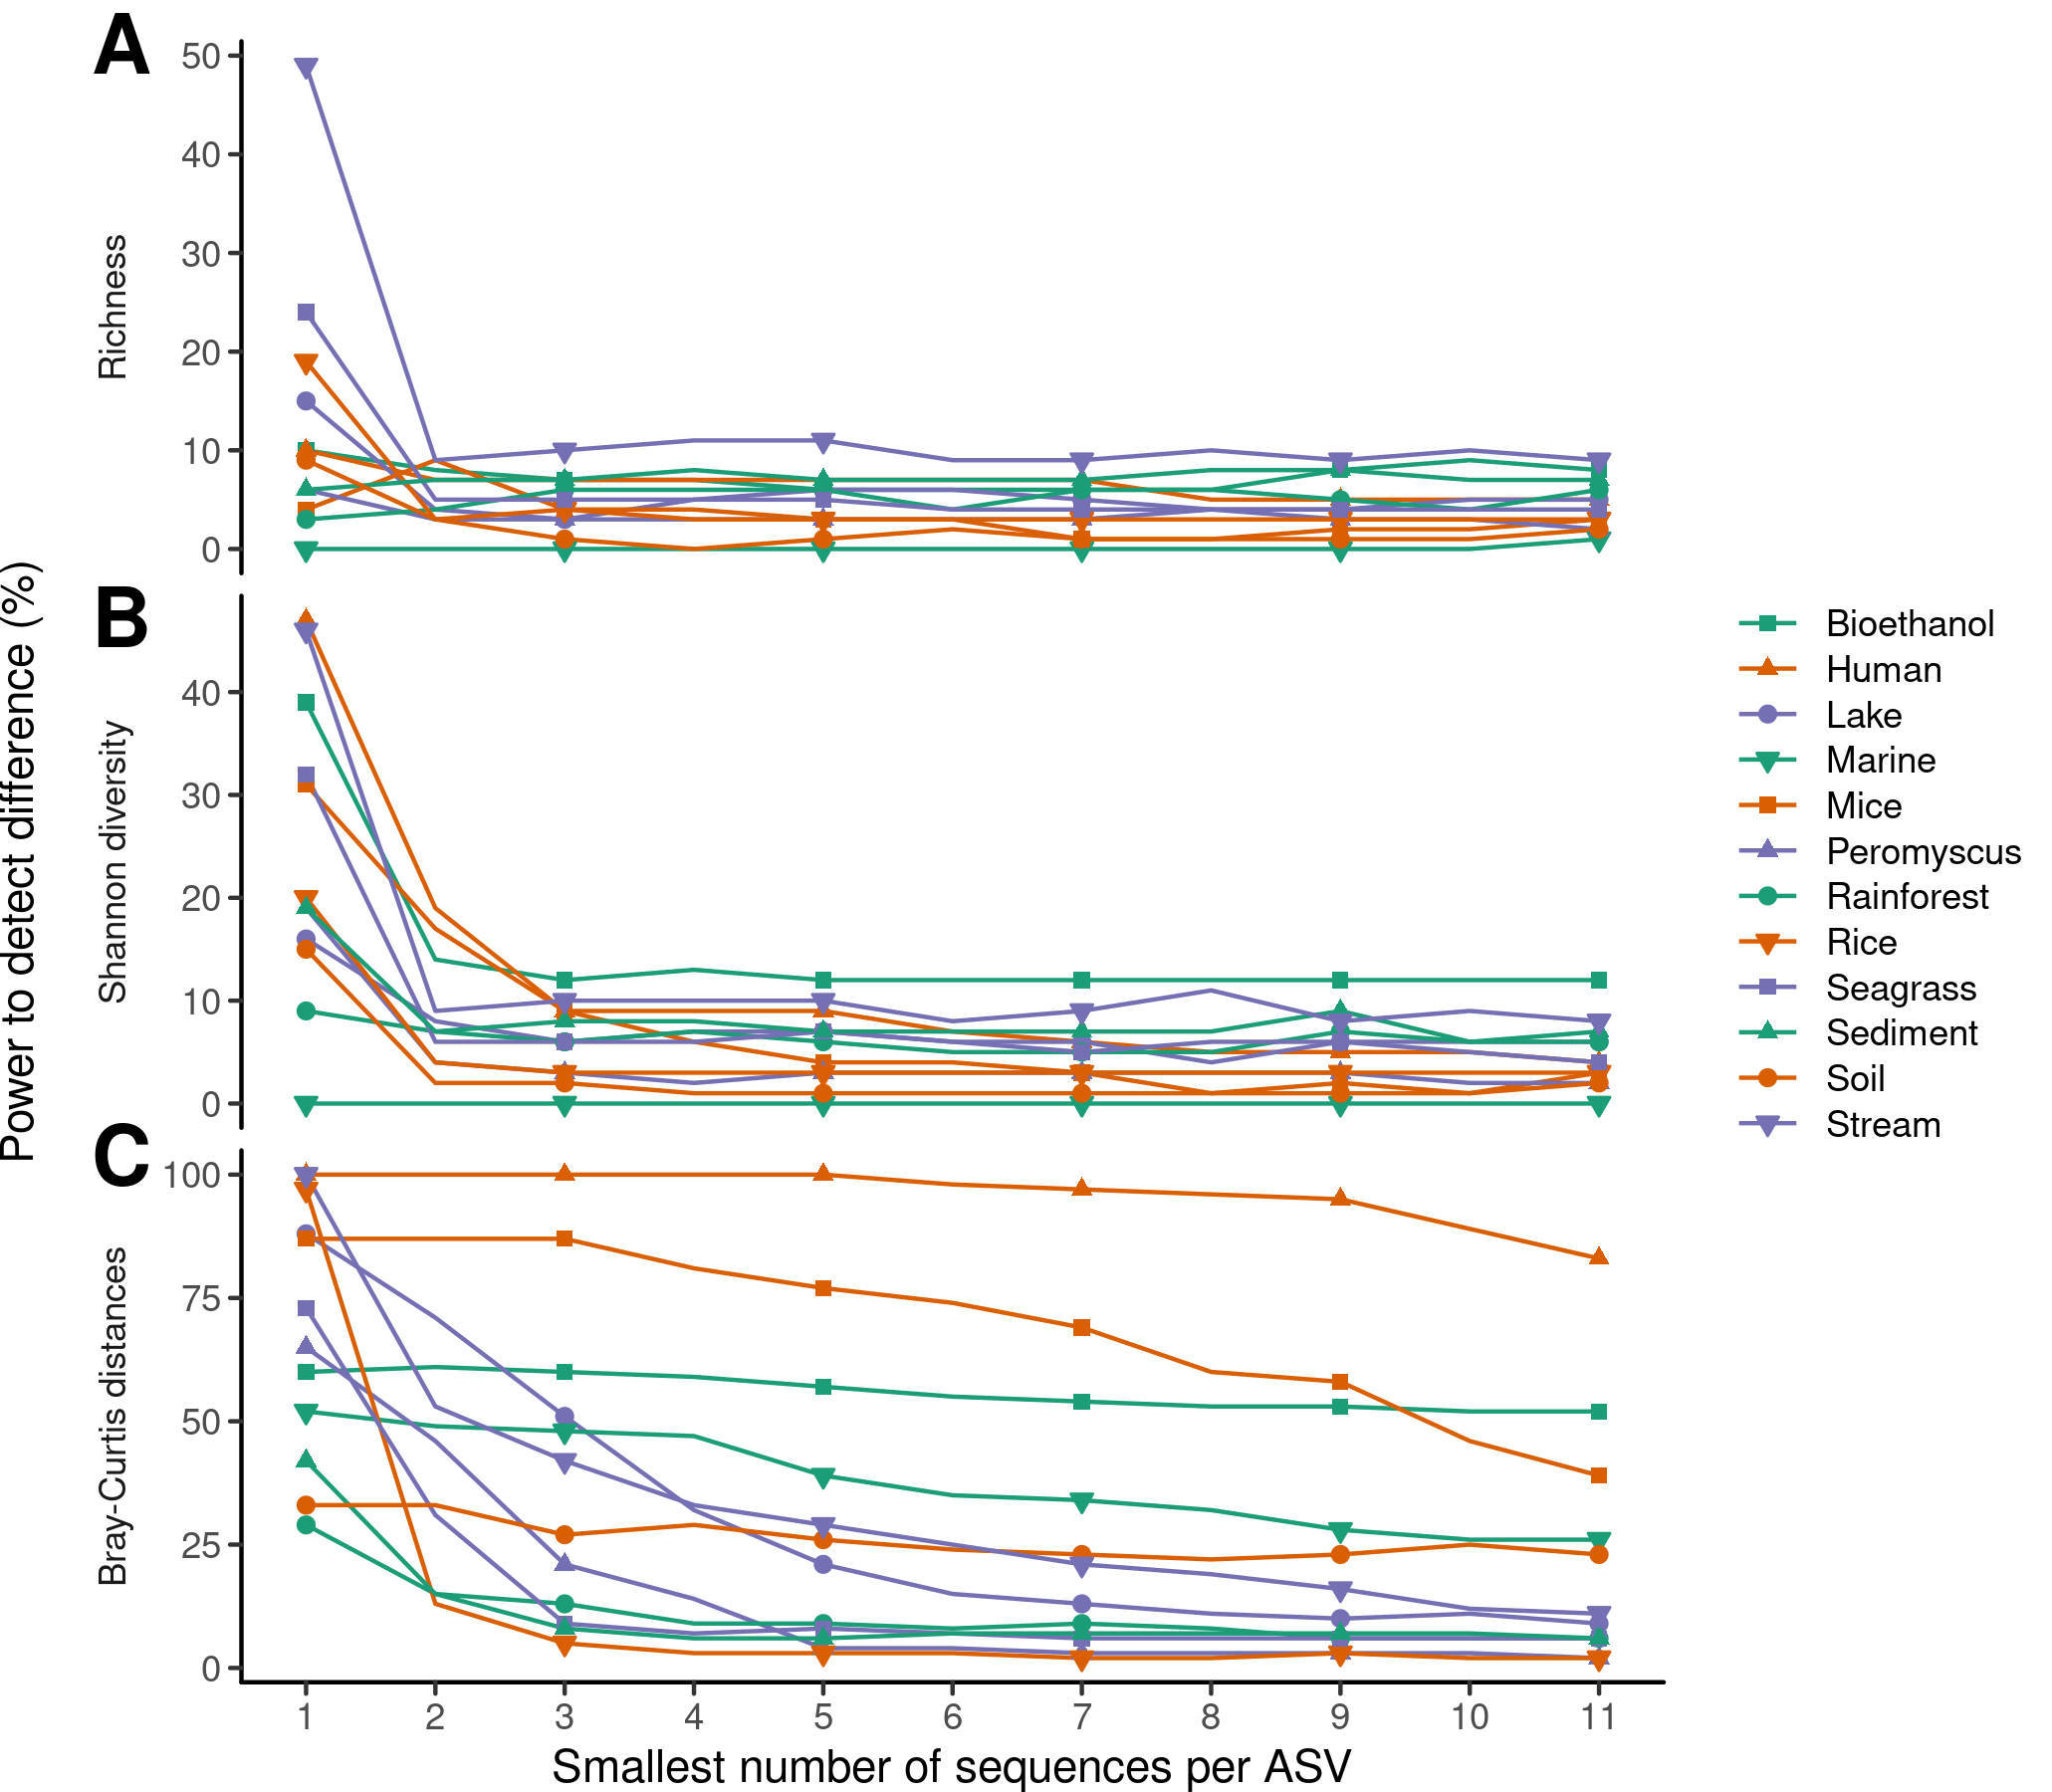
\includegraphics{figure_s5.png}

\textbf{Figure S5. Removing rare sequences from samples reduces the
statistical power to detect differences between empirically generated
treatment groups when using operational taxonomic units (OTUs).} The
fraction of significant tests comparing the richness (A) and Shannon
diversity (B) using a Wilcox test and Bray-Curtis distances (C) using
analysis of molecular variance for each dataset was calculated using
empirically generated treatment groups containing equal numbers of
samples for each dataset with varying minimum abundance thresholds. For
each dataset and minimum abundance threshold, 100 randomizations were
peformed.

\newpage

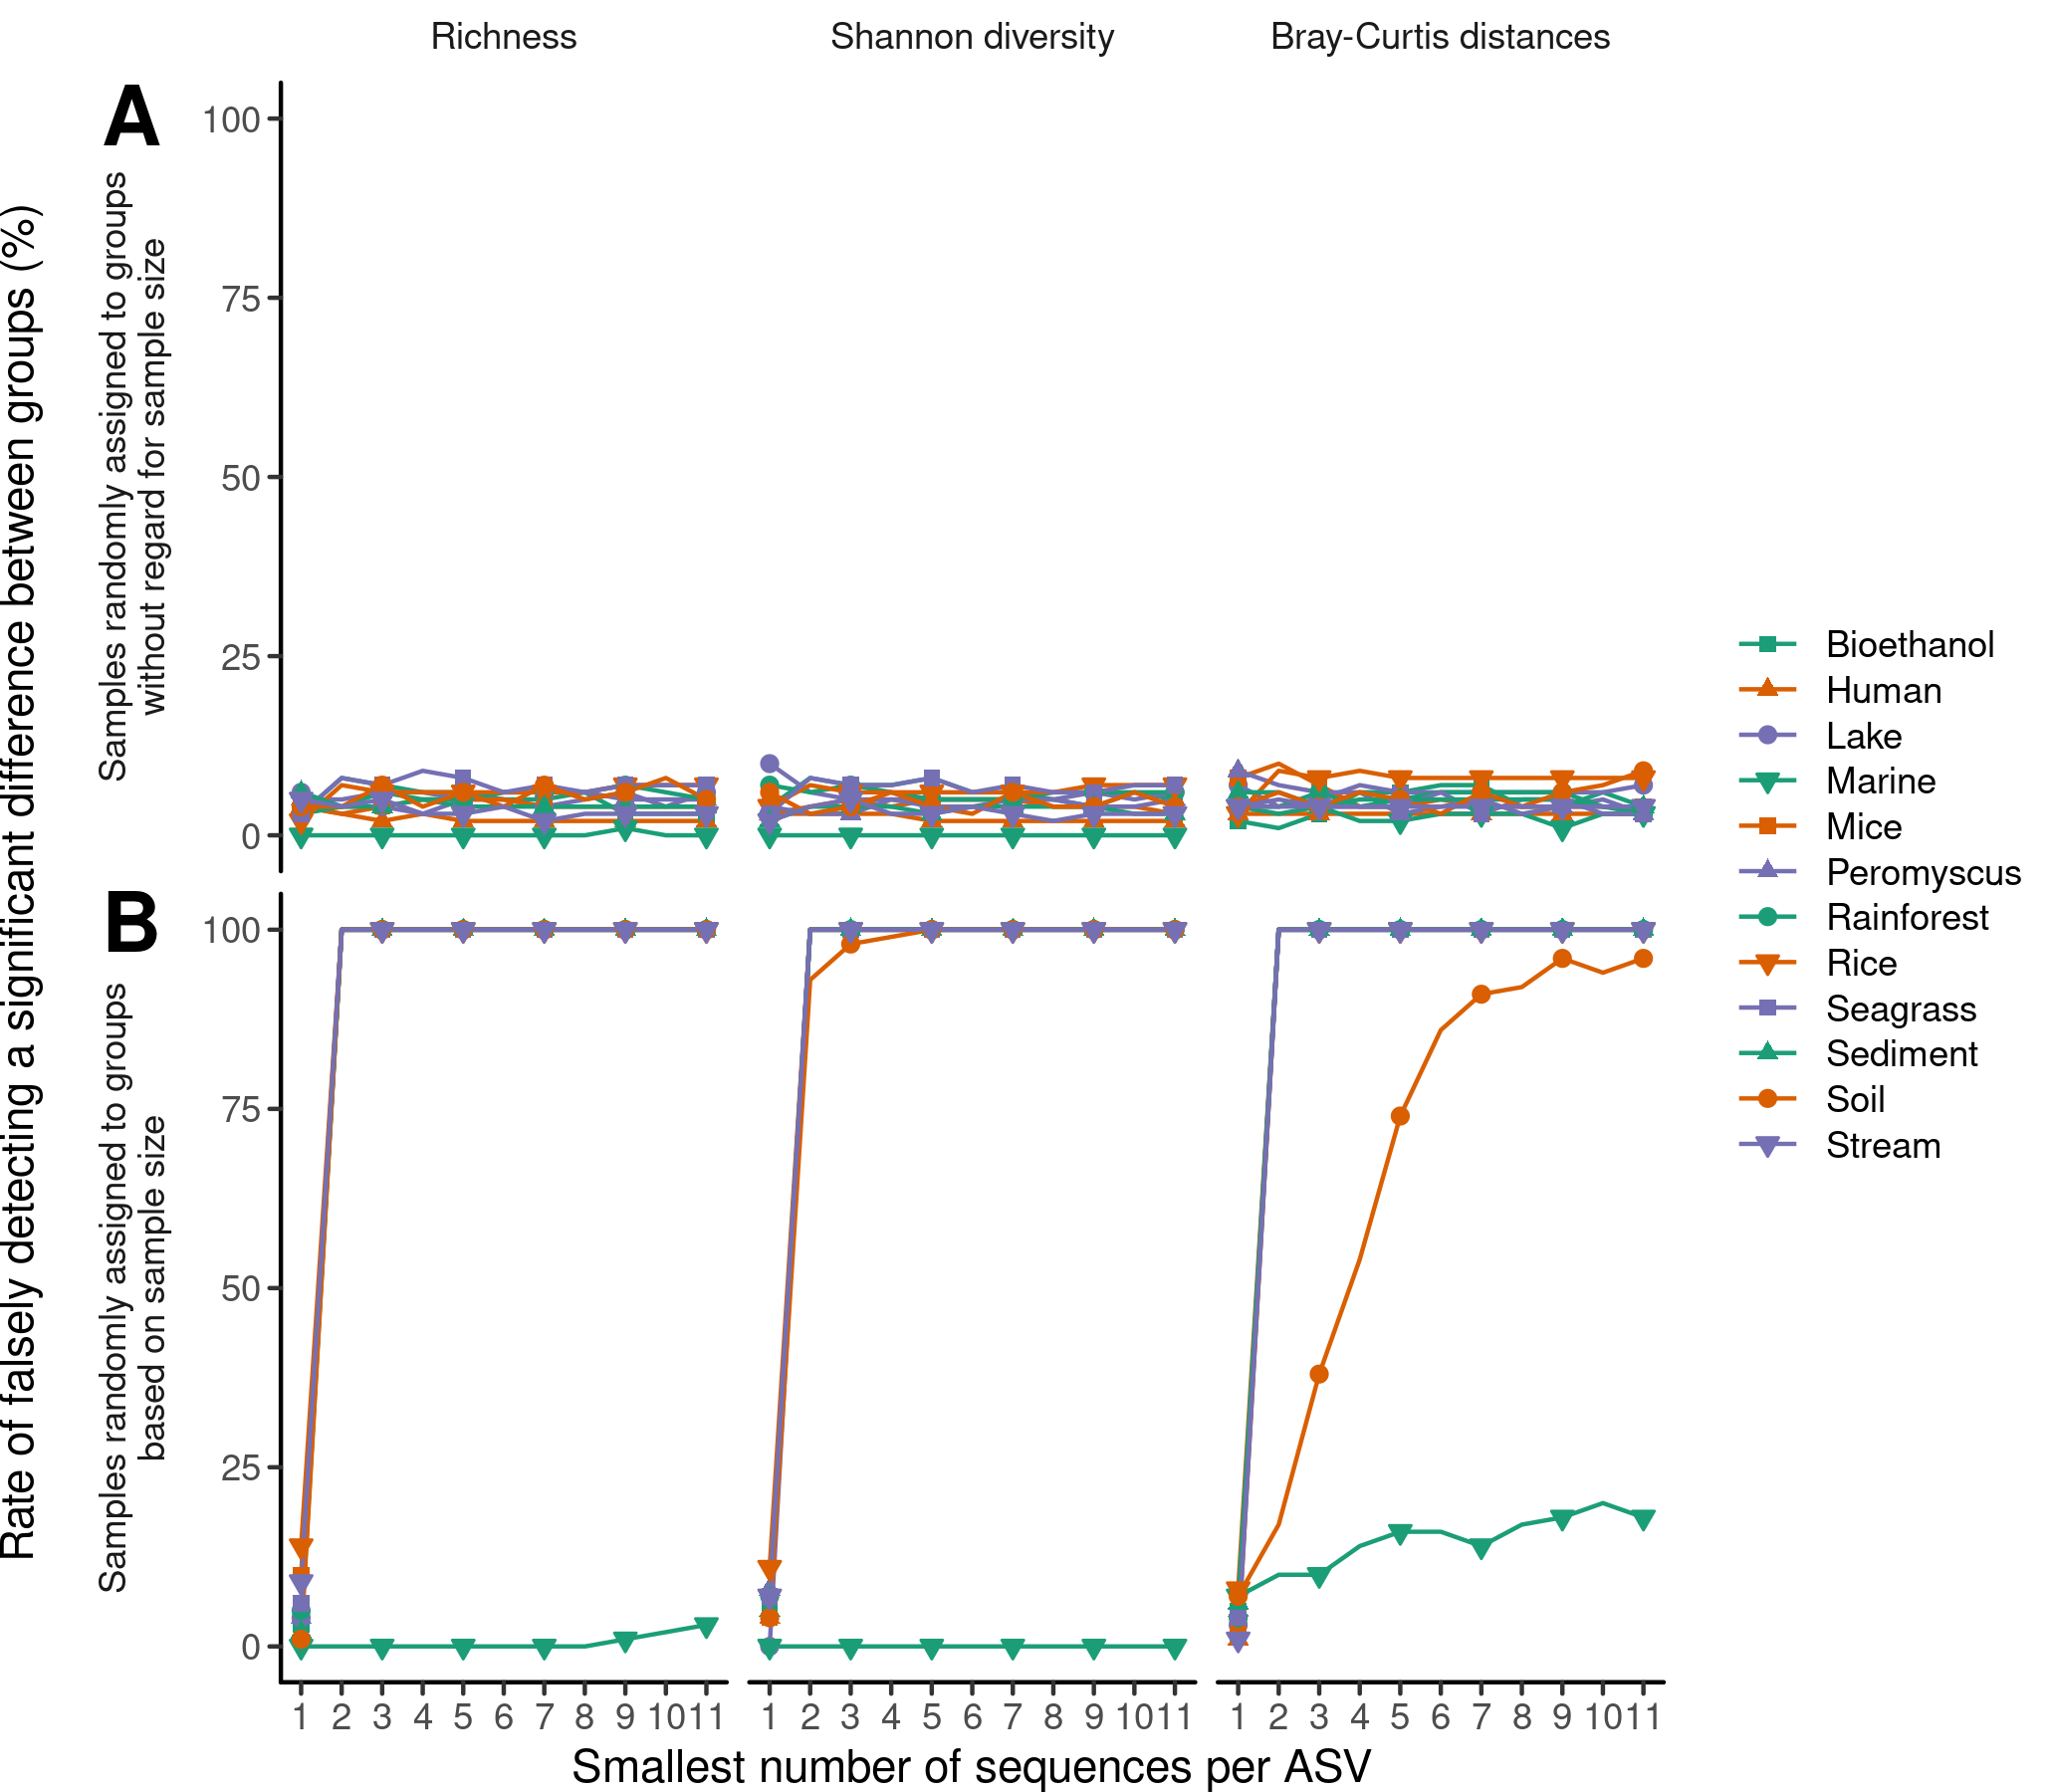
\includegraphics{figure_s6.png}

\textbf{Figure S6. Removing rare sequences does not impact the false
detection rate unless the number of sequences per sample is confounded
with the treatment groups when using operational taxonomic units
(OTUs).} The fraction of significant tests comparing the richness and
Shannon diversity using a Wilcox test and Bray-Curtis distances using
analysis of molecular variance for each dataset was calculated.
Empirically generated treatment groups were generated containing equal
numbers of samples where the samples represented a null distribution. In
one simulation the samples were randomly assigned to a treatment group
(A) and in the other the samples were assigned based on the number of
sequences in each sample (B). For each dataset and minimum abundance
threshold, 100 randomizations were peformed.

\end{document}
